\documentclass{VUMIFPSbakalaurinis}
\usepackage{algorithmicx}
\usepackage{algorithm}
\usepackage{algpseudocode}
\usepackage{amsfonts}
\usepackage{amsmath}
\usepackage{bm}
\usepackage{caption}
\usepackage{color}
\usepackage{float}
\usepackage{graphicx}
\usepackage{listings}
\usepackage{subfig}
\usepackage{wrapfig}
\usepackage{enumitem}
\usepackage{longtable}
\usepackage{multirow}
\usepackage{multicol}

\setitemize{noitemsep,topsep=0pt,parsep=0pt,partopsep=0pt}
\setenumerate{noitemsep,topsep=0pt,parsep=0pt,partopsep=0pt}

% Titulinio aprašas
\university{Vilniaus universitetas}
\faculty{Informatikos institutas}
\department{Programų sistemų katedra}
\papertype{Bakalauro baigiamasis darbas}
\title{Mažos duomenų imties problemos poveikis klasifikacijos tikslumui naudojant dirbtinius neuroninius tinklus}
\titleineng{The Effect of a Small Dataset Problem on Classification Accuracy Using Artificial Neural Networks}
\author{Miglė Vaitulevičiūtė}
\supervisor{asist. dr. Vytautas Valaitis}
\reviewer{j. asist. Linas Petkevičius}
\date{Vilnius – \the\year}

% Nustatymai
% \setmainfont{Palemonas}   % Pakeisti teksto šriftą į Palemonas (turi būti įdiegtas sistemoje)
\bibliography{bibliografija}

\begin{document}
\maketitle
\cleardoublepage\pagenumbering{arabic}
\setcounter{page}{2}
\tableofcontents

\sectionnonum{Santrauka}
Šį darbą sudaro teorinė ir eksperimentinė dalys. Teorinėje dalyje pirmiausia yra aprašomas dirbtinis neuroninis tinklas, jo sudėtis ir veikimas. Toliau yra apibrėžiami konvoliuciniai neuroniniai tinklai, jų sudėtis bei esamos architektūros. Taip pat yra apibrėžiamas AutoML ir architektūros paieškos algoritmas, kadangi eksperimentinėje dalyje yra naudojamas NASNet modelis. Šis modelis buvo pasirinktas dėl savo inovatoriškumo bei AutoML panaudojimo. 
Eksperimentinėje dalyje du NASNet modeliai (NASNet Large ir NASNet Mobile) yra suderinami su dviem skirtingais mažo kiekio duomenų rinkiniais bei keičiant mokomų sluoksnių kiekį. Naudojami du NASNet modeliai, nes jų gyliai skiraisi ir taip galima pamatyti kokią įtaką modelio gylis daro tikslumui. Gauti bandymų rezultatai lyginami, pateikiamos išvados.

\raktiniaizodziai{NASNet, AutoML, derinimas, konvoliuciniai neuroniniai tinklai, neuroninės architektūros paieškos algoritmas, tikslumas, mažos duomenų imties problema}

\sectionnonum{Summary}
This work consists of theoretical and experimental parts.  The theoretical part firstly describes the artificial neural network, its structure and functioning. Next, convolutional neural networks, their composition and existing architecture are defined. Also, the AutoML and architecture search algorithm are defined, as the NASNet model is used in the experimental part. This model has been chosen for its innovation and the use of AutoML.
In the experimental part, two NASNet models (NASNet Large and NASNet Mobile) are fine-tuned with two different small datasets while changing the number of training layers. Two NASNet models are used, because they differ in depth and can be used to see the impact of model depth on accuracy. The obtained test results are compared and conclusions are given.

\keywords{NASNet, AutoML, fine-tune, convolutional neural networks, neural architecture search algorithm, accuracy, small dataset problem}

\sectionnonum{Įvadas}

Vienas iš dirbtinių neuroninių tinklų tipų yra konvoliuciniai neuroniniai tinklai, kurių viena iš sprendžiamų problemų yra klasifikacijos uždavinys \cite{fukushima, LeCun:1999:ORG:646469.691875}. 
Tai yra procesas, kurio metu yra ieškoma panašių požymių (angl. feature) tarp skirtingų objektų, pavyzdžiui, 
paveiksliukų, ir pagal tai jie yra skirstomi į atitinkamas klases \cite{classificationDef}. Klasifikacija yra labai aktuali, kadangi ji yra naudojama 
nuo medicinos iki savivaldžių automobilių. 

Konvoliuciniai neuroniniai tinklai gali būti naudojami:
\begin{itemize}
    \item Veido atpažinimui - identifikuoti arba verifikuoti asmenį. Pavyzdžiui, „DeepFace“ sistema sukurta „Facebook“ \cite{Taigman:2014:DCG:2679600.2680208}, kuri atpažįsta žmonių veidus nuotraukose, 
arba „Face ID“ sistema sukurta „Apple“, kuri yra skirta identifikuoti asmenį, kuris bando atrakinti telefoną. 
    \item Medicinoje - širdies, plaučių, prostatos, krūties vėžių \cite{cancer}, akių ligų diagnozavimui \cite{eyedis}.
    \item Žmonių elgesio analizė realiu laiku – „DeepGlint“ nustato žmones nuotraukose ir nuspėja jų elgesį \cite{deepGlint}.
    \item Vertimas – „Google Translate“ gali versti tekstą iš paveiksliukų realiu laiku \cite{Raschka:2015:PML:2886323}.
\end{itemize}

Tam kad neuroninius tinklus būtų galima panaudoti kažkokioje sferoje reikia turėti neuroninių tinklų ekspertą bei tinkamai sužymėtą ir didelį duomenų rinkinį (angl. dataset). 
Mokslininkai ir komercinės įmonės neturinčios žinių neuroninių tinklų ar mašininio mokymosi srityse negali pasinaudoti jų teikiamais privalumais, nes egzistuoja per daug kintamųjų, pavyzdžiui, architektūros pasirinkimas, hiperparametrų optimizavimas, 
kurie lemia ar tinklas gerai atliks jam paskirtą užduotį \cite{14f00e7a0861477a81f65b5c51f660f4, DBLP:journals/corr/abs-1902-06827}. Taip pat visiems neuroniniams tinklams reikia didelio kiekio duomenų, kadanagi jų tikslumas didėja logaritmiškai \cite{DBLP:journals/corr/ChoLSCD15, DBLP:journals/corr/SunSSG17}. 
Tačiau realiame pasaulyje duomenų kiekis ir žmogiškieji bei laiko resursai yra riboti, todėl yra siekiama keičiant dirbtinio tinklo architektūrą bei jo parametrus gauti kuo didesnį tikslumą. Tad, architektūros paieškos ir parametrų 
nustatymo automatizavimas turėtų leisti pigiau ir greičiau sukurti efektyvų bei tikslų neuroninį tinklą negu kad tai darant rankiniu būdu \cite{DBLP:journals/corr/RealMSSSLK17}.
Tokiam procesui atlikti yra naudojamas automatizuotas mašininis mokymasis (angl. Automated Machine Learning (toliau - AutoML)).

2017 metais Google komanda naudodami AutoML sukūrė naują architektūrą NASNet \cite{DBLP:journals/corr/ZophVSL17}, kuri yra sudaryta iš dviejų tipų blokų, kurie yra sudėti vienas ant kito. 
Šiai architektūrai sukurti buvo naudojamas neuroninės architektūros paieškos (angl. neural architecture search) algoritmas. Jis automatiškai keisdamas vidinius parametrus ieško geriausios architektūros specifiniai duomenų imčiai.
Taip pat NASNet modelio tikslumas yra 1,2\% didesnis negu bet kokios kitos žmogaus sukurtos architektūros \cite{DBLP:journals/corr/ZophVSL17}.

Bakalauro darbo tikslas yra palyginti skirtingų gylių NASNet modelių veikimą su mažu duomenų rinkiniu.

Uždaviniai:
\begin{enumerate}
    \item Apžvelgti dirbtinių neuroninių tinklų ir konvoliucinių neuroninių tinklų sudėtį bei NAS algoritmo veikimą.
    \item Rasti geriausius hiperparametrus skirtingų gylių modeliams su pasirinktu mažu duomenų rinkiniu.
    \item Suderinti (angl. fine-tune) egzistuojančius skirtingų gylių modelius su pasirinktu mažu duomenų rinkiniu.
    \item Palyginti ir įvertinti skirtingų gylių modelius pagal gautą derinimo informaciją.
\end{enumerate}

\section{Dirbtinis neuroninis tinklas}
Pagal apibendrintą žmogaus smegenų veikimą buvo sugalvoti dirbtiniai neuroniniai tinklai \cite{Goodfellow-et-al-2016}. Bendrai žmogaus smegenys turi šimtus
milijardų neuronų, kurie yra sujungti sinapsėmis. Per šiuos neuronus sklinda elektroniniai impulsai, perduodantys informaciją. Tokiu būdu žmonės gali 
atpažinti objektus, garsus ir t.t. Dirbtiniai neuroniniai tinklai veikia panašiai. Jie turi daug besijungiančių neuronų, kurie gauna informaciją ir 
pagal tą informaciją gali nuspręsti koks tai objektas. Tačiau ties tuo ir baigiasi žmogaus smegenų ir dirbtinių neuroninių tinklų panašumas, 
kadangi dirbtiniai neuroniniai tinklai yra matematinis algoritmas su aritmetiniais kintamaisiais. Šis algoritmas yra suvokiamas 
tik žmogui, kuris suprogramavo dirbtinį neuroninį tinklą, pačiam tinklui algoritmas nieko nereiškia, nuovokos nesuteikia.

\subsection{Dirbtinio neuroninio tinklo sudėtis}
Dirbtinis neuroninis tinklas yra sluoksnių rinkinys - neuronų grupė sudaro sluoksnį, kuris yra sujungtas tarpusavyje su kitais sluoksniais \cite{1193152}. Vienas iš
sluoksnių privalo būti įvesties sluoksnis, kuris atitinkamai pagal užduotį gali gauti įvairios formos informaciją - paveiksliukai, vaizdo
medžiaga, garsas ir t.t. Ši informacija yra reikalinga tam, kad tinklas galėtų ją išanalizuoti ir išmokti, kad vėliau gavęs panašią
informaciją galėtų ją atpažinti - tam reikalingas išvesties sluoksnis. Jis yra priešingame dirbtinio neuroninio tinklo gale negu įvesties sluoksnis.
Tarp anksčiau apibūdintų sluoksnių yra įvairaus dydžio vidinė sluoksnių sistema, kuri atlieka pagrindinį darbą.

\subsection{Dirbtinio neuroninio tinklo veikimas}
Jungtys tarp neuronų yra pateiktos skaitine išraiška ir vadinamos svoriu. Kuo didesnis šis svoris tuo didesnę įtaką turi vienas neuronas kitam.
Vienam neuronui yra pateikiama visų prieš jį buvusių neuronų informacija ir jungčių svoriai. Kiekvieno neurono informacija yra sudauginama su
jo svoriu ir visi šie duomenys yra sudedami tarpusavyje bei pridedama slenksčio reikšmė (angl. bias). Taip iš vektoriaus gaunamas vienas rezultatas ir jei šis rezultatas tinka aktyvavimo
funkcijai, jis yra perduodamas tolimesniems neuronams \cite{shiffman2012nature}. Tokio tipo veikimo projektavimas yra vadinamas tiesioginio sklidimo (angl. feedforward) tinklu.

Tačiau jungčių svoriai nėra pastovūs. Kai dirbtinis neuroninis tinklas mokosi, galutinis rezultatas yra lyginamas su tikėtinu teisingu rezultatu (daugiau informacijos „Nuostolio funkcija“), jei šie
rezultatai skiriasi, slenksčio reikšmės ir svoriai yra keičiami atitinkamai \cite{backpropogation}, tai vadinama sklidimo atgal algoritmu (angl. backpropagation).
Mokymo metu duomenys neuroniniu tinklu keliauja į priekį - nuo įvesties į išvesties sluoksnį. Kai išvesties sluoksnis yra pasiekiamas, gautas rezultatas yra palyginamas su norimu rezultatu bei 
apskaičiuojama nuostolio funkcija - kaip stipriai skiriasi gautas ir norimas rezultatai. Pagal šią reikšmę matoma, kaip reiktų keisti gautą rezultatą, kad nuostolio funkcijos reikšmė pasiektų lokalų 
minimumą. Tačiau siekiant aukštesnio tikslumo reikia keisti viso neuroninio tinklo parametrus - svorius, slenksčio reikšmes. Taigi, iš išvesties rezultatų galima matyti, kaip reikia pakeisti - 
didinti arba mažinti - prieš tai buvusio sluoksnio parametrus, kad būtų gautas geriausias tikslumas. Šis procesas yra iteratyviai kartojamas kiekvienam neuronui su prieš jį einančiu sluoksniu bei jį galima įvardinti kaip funkciją (1):
\begin{equation}
\frac{\partial{C_{0}}}{\partial{w^{L}}} = \frac{\partial{z^{L}}}{\partial{w^{L}}} \frac{\partial{a^{L}}}{\partial{z^{L}}} \frac{\partial{C_{0}}}{\partial{a^{L}}}.
\end{equation}
Šioje funkcijoje vienas sluoksnis turi vieną neuroną, priklausomai nuo neuronų ir sluoksnių skaičiaus prie funkcijos parametrų prisidėtų atitinkami indeksai. Funkcija parodo dalinės nuostolio funkcijos 
išvestinės ir dalinės svorio (arba slenksčio reikšmės) išvestinės santykį, kur \(w^{L}\) yra svoris, kurį galima pakeisti į \(b^{L}\) (slenksčio reikšmė), \(C_{0}\) yra nuostolio funkcijos reikšmė, 
\(z^{L} = w^{L}a^{L-1}+b^{L}\) ir \(a^{L}=\sigma(z^{L})\). Šitos funkcijos tikslas yra nustatyti kokį efektą svorio reikšmės pakeitimai turės nuostolio funkcijos reikšmei.

\subsection{Aktyvavimo funkcijos}
Aktyvavimo funkcijų (angl. activation function) yra įvairių, todėl specifinės problemos gali reikalauti vienos ar daugiau konkrečių aktyvavimo funkcijų \cite{activation}.
Aktyvavimo funkcija yra skirta tam, kad nustatytų ar neuronui reikia būti aktyvuotam ar ne. Tai yra nusprendžiama pagal duomenis, kuriuos neuronas gauna, jeigu jie yra aktualūs, neuronas yra aktyvuojamas, jeigu ne - ignoruojamas.
Šią funkciją galima aprašyti žemiau pateikta formule (2):
\begin{equation}
Y = A(\Sigma{(w * d) + b}).
\end{equation}

Formulėje (2) pateikta raidė \(A\) reiškia bet kokia pasirinkta aktyvavimo funkcija, o jos parametrai \(w\) yra svoris, \(d\) yra įvesties duomenys ir \(b\) yra slenksčio reikšmė. Taigi, ar neuronas bus aktyvuotas priklauso nuo prieš jį 
buvusio sluoksnio jungčių dydžio, kurios parodo kiek svarbi yra jungtis tarp neuronų, kadangi kuo didesnis svoris tuo didesnis rezultatas gaunamas svorį sudauginus su įvesties duomenimis. Taip pat slenksčio reikšmė parodo ar reikia 
sustiprinti ar susiplinti gaunamą rezultatą. \(Y\) reikšmė priklauso nuo pasirinktos aktyvavimo funkcijos išvesties intervalo. Žemiau yra pateiktos kelios aktyvavimo funkcijos su išvesties intervalais.  

Kelios aktyvavimo funkcijos:
\begin{itemize}
\item Sigmoidinė (angl. sigmoid function) - išvesties intervale [0; 1].
\item Hiperbolinio tangento (angl. hyperbolic tangent) - išvesties intervale [-1; 1].
\item Minkštojo maksimumo (angl. softmax function) - sunormuoja išvesties vektorių į 1.
\item ReLU - išvesties intervale [0; begalybė].
\end{itemize}

\subsection{Nuostolio funkcijos}
Mokantis dirbtiniam neuroniniam tinklui jo gaunami rezultatai gali labai skirtis nuo tikėtinų rezultatų, todėl nuostolio funkcija apskaičiuoja kaip stipriai
skiriasi gautas rezultatas nuo tikėtino. Kuo didesnis nuostolis tuo toliau nuo teisingo atsakymo yra dirbtinis neuroninis tinklas \cite{Cameron-loss-fun}.
Paprasčiausia ir dažniausiai naudojama nuostolio funkcija yra vidutinio kvadratinio nuokrypio (angl. mean squared error). Ši funkcija apskaičiuoja kvadratinį skirtumą tarp tikėtino 
ir gauto rezultatų. Tačiau šios funkcijos vienas iš didesnių trūkumų - neproporcingas išskyrimas didelių rezultatų. Kadangi funkcija didėja kvadratiškai,
o ne tiesiškai, tai gaunamas rezultatas tolsta nuo tikėtino rezultato.

Priklausomai nuo to kokią problemą yra bandoma išspręsti yra naudojamos skirtingos funkcijos. Viena iš problemų yra klasifikacijos - dažniausiai išvesties
rezultatas yra tikimybės vertė f(x). Bendrai, funkcijos reikšmės dydis parodo gauto rezultato tikslumą.

Kelios klasifikacijos nuostolio funkcijos:
\begin{itemize}
\item Binarinė kryžiaus entropija (angl. binary cross entropy).
\item Neigiama registravimo tikimybė (angl. negative log likelihood).
\item Maržos klasifikatorius (angl. margin classifier).
\item Minkštų maržų klasifikatorius (angl. soft margin classifier).
\end{itemize}

\subsection{Optimizavimo funkcijos}
Optimizavimo funkcijos naudojamos vidinių tinklo parametrų atnaujinimui, kad sumažinti gaunamų rezultatų netikslumą \cite{Niknafs2016NeuralNO}. 
Visos optimizavimo funkcijos gali būti suskirstytos į du tipus - nuolatinio mokymosi greičio ir prisitaikančio mokymosi. 
Lentelė 1 buvo parengta remiantis \cite{DBLP:journals/corr/Ruder16} straipsniu. Lentelėje išvardintos visos populiariausios optimizavimo funkcijos.

\begin{longtable}[h!]{ | p{2cm} | p{2.2cm} | p{2.5cm} | p{2.5cm} | p{4.5cm} | } 
\caption{Optimizavimo funkcijos} \\ \hline
Pavadinimas & Tipas & Privalumai & Trūkumai & Veikimas \\ \hline
\endhead
SGD & Nuolatinio mokymosi greičio & Parametrų atnaujinimai turi aukštą dispersiją, kas leidžia lengviau rasti lokalų minimumą. & Didelis svyravimas trukdo konverguoti. & Parametrų atnaujinimas vykdomas kiekvienai mokymo iteracijai. \\ \hline
Adam & Prisitaikančio mokymosi & Greitai konverguoja ir modelio mokymosi greitis yra didelis bei efektyvus. & Praleidžia mažą lokalų minimumą. & Suskaičiuoja mokymosi greitį kiekvienam parametrui bei saugo eksponentiškai nykstantį prieš tai buvusį kvadratinio gradiento vidurkį ir eksponentiškai mažėjantį prieš tai buvusį gradiento vidurkį, panašų į pagreitį. \\ \hline
Adagrad & Prisitaikančio mokymosi & Nereikia rankiniu būdu derinti mokymosi greičio. & Mokymosi greitis visada yra mažėjantis ir nykstantis, kas lėtina konvergavimą. & Leidžia mokymosi greičiui priklausyti nuo parametrų. Dideli atnaujinimai nedažniems parametrams, maži atnaujinimai dažniems parametrams. \\ \hline
RMSprop & Prisitaikančio mokymosi & Greitai konverguoja. & Pagreitis (angl. momentum) nedidina funkcijos efektyvumo. & Dalija mokymosi greitį iš eksponentiškai nykstančio kvadratinio gradiento vidurkio. \\ \hline
\end{longtable}

Skyriuje „Dirbtinio neuroninio tinklo veikimas“ minėta, kad sklidimo atgal algoritmas pagal gauto ir norimo 
rezultatų skirtumą keičia vidinius neuroninio tinklo parametrus. Vidinių parametrų atnaujinimui yra naudojama 
optimizavimo funkcija, kuri apskaičiuoja gradientą. Svoriai yra keičiami pagal priešingą apskaičiuoto gradiento 
kryptį - bandoma leistis į gradiento minimumą.

Optimizavimo funkcijos turi parametrą - mokymosi greitį (angl. learning rate). Jis privalo būti nustatytas, tačiau 
pasirinkti tinkamą mokymosi greitį gali būti sudėtinga - pasirinkus per mažą vidiniai parametrai gali labai lėtai 
konverguoti, o pasirinkus per didelį - parametrams gali trukdyti konverguoti ir priversti nuostolio funkciją svyruoti
apie minimumą arba diverguoti \cite{leondes1998image}. Optimizavimo funkcijos tikslas yra surasti lokalų minimumą, 
o to pasiekti galima gradientu judant į žemiausią jo vietą, tačiau pasirinkus per didelį mokymosi greitį yra galimybė, 
kad žemiausia vieta bus peršokta ir bus tolstama nuo jos.

\subsection{Hiperparametrai}

Mašininame mokymesi terminas hiperparametras (angl. hyperparameter) yra naudojamas atskirti parametrus, kurie nėra išmokstami iš duomenų, kurie yra naudojami mokant modelį. Hiperparametrai apima kintamuosius skirtus reguliuoti neuroninį tinklą. Jie turi labai didelį poveikį neuroninio tinklo tikslumui, tačiau pasirinkti jų vertes gali būti sudėtinga, nes įtaką daro architektūra, duomenų rinkinys. Optimalių hiperparametrų radimui yra sugalvota daug metodų, kurie yra aprašyti „Paieškos strategija“ skyriuje. 
Dalis hiperparametrų yra: mokymosi greitis, epochų ir partijų (angl. batch) vertės, vidinių sluoksnių kiekis, išmetimo sluoksnio reikšmė, aktyvacijos, optimizacijos ir nuostolio funkcijos. 

\section{Konvoliucinis neuroninis tinklas}
Konvoliuciniai neuroniniai tinklai yra labai panašūs į paprastus dirbtinius neuroninius tinklus (daugiau informacijos skyriuje „Dirbtinis neuroninis
tinklas“). Tačiau pagrindinis skirtumas tarp šių tinklų yra, kad konvoliucinio neuroninio tinklo įvesties sluoksnis priima duomenis, kurie gali būti konvertuojami į 2D matricą, pavyzdžiui, paveiksliukai, 
kurie jei padaryti su standartine skaitmenine kamera, turi tris komponentus - raudoną, žalią ir mėlyną. Šiuos komponentus galima 
įsivaizduoti kaip tris 2D matricas sudėtas viena ant kitos. Kiekvienos matricos i-osios eilutės ir j-ojo stulpelio elementas 
atitinka nuotraukos pikselį, kurio reikšmė yra intervale nuo 0 iki 255. Kadangi naudojamos informacijos tipas yra specifinis, 
tai labai sumažina tinklo parametrų kiekį ir tinklą padaro efektyvesnį \cite{CnnImages}.

Objektų atpažinimas paveiksliukuose yra sudėtingas dėl šių iššūkių:
\begin{itemize}
\item Segmentavimas - paveiksliukai gali atvaizduoti įvairias scenas, kuriose gali būti pavaizduota daug objektų, kurie vienas kita gali dalinai uždengti.
\item Šviesa - pikselių intensyvumas gali būti paveiktas šviesos šaltinio ar pačio objekto.
\item Deformacija - objektai gali būti deformuoti įvairiais būdais, pavyzdžiui, kiekvieno žmogaus ranka parašyti skaičiai skiriasi.
\item Galimybės - objektų klasės dažnai nustatomos pagal tai kaip patys objektai yra naudojami, pavyzdžiui, kėdės yra objektai sukurti sėdėti, tačiau jos gali turėti skirtingus dizainus.
\item Žvilgsnio taškas - keičiant vietą iš kurios yra žiūrima gali keistis objekto forma, informacija šokinėja per įvesties sluoksnio dimensiją (t.y. pikselius). 
\end{itemize}

\subsection{Konvoliucija}
Konvoliucija yra matematinė operacija, kuri apibūdina taisyklę, kuri parodo kaip reikia sujungti du informacijos rinkinius \cite{Convolution-book}. 

\begin{figure}[h]
    \centering
    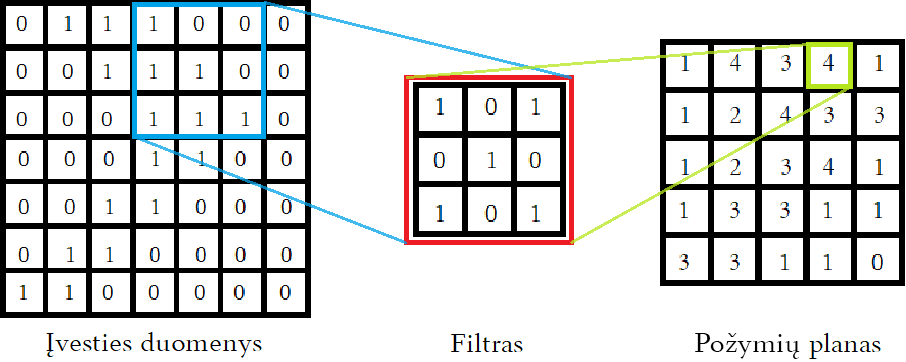
\includegraphics[width=1\textwidth]{img/matrica.png}
    \caption{Konvoliucijos veikimas}
\end{figure}

Pagal paveiksliuką (1 pav.) matyti, kad įvesties duomenys ir filtras, kuris yra sudarytas iš svorių, yra pateikti 2D matrica. Filtras juda nuo duomenų matricos kairės viršutinės dalies į dešinę, 
tada yra nuleidžiamas žemiau per vieną eilutę ir taip filtras juda per visą duomenų matricą, kol su visais jos duomenimis filtras yra sudauginamas ir užpildo naują matricą, kuri 
yra vadinama požymių planu (angl. feature map).
Tačiau konvoliuciniai tinklai turi daug filtrų, kurie pereina per vieną paveiksliuką, kiekvienas išskirdamas skirtingą paveiksliuko požymį \cite{DBLP:journals/corr/abs-1708-08711}.
Pirmuose sluoksniuose šiuos filtrus galima apibūdinti kaip horizontalių, vertikalių ar įstrižų linijų filtrus, kurie sukuria paveikslėlio 
kraštų planą.

\subsection{Konvoliucinio neuroninio tinklo sluoksniai}
Konvoliuciniai neuroniniai tinklai tai yra sluoksnių rinkinys, kuris turi įvesties, vidinius ir išvesties sluoksnius. Tačiau priklausomai 
kokio tipo konvoliucinis neuroninis tinklas vidiniai sluoksniai gali skirtis. Konvoliuciniai neuroniniai tinklai turi tris pagrindinius 
sluoksnių tipus, kurie sudaro vidinį sluoksnį. Šie tipai yra konvoliucinis, sujungimo ir pilno sujungimo sluoksniai \cite{CNNbasic}.

Nepagrindinių sluoksnių paaiškinimai:
\begin{itemize}
\item Plokštinimo sluoksnis (angl. flatten layer) - skirtas tam, kad įeinančius duomenis suploti į atitinkamą sluoksnių skaičių, jeigu sluoksnio parametras nenustatytas suplojama į vieną sluoksnį.
\item Išmetimo sluoksnis (angl. dropout layer) - sluoksnyje atsitiktinai yra išjungiami tam tikri neuronai su Bernulio pasiskirstymo tikimybe, kuri priima dvi reikšmes 1 (sėkmė) ir 0 (nesėkmė) 
bei šių reikšmių tikimybe \(p\) ir \(1 - p\). Dažniausiai yra nustatytas 50 procentų.
\end{itemize}

\subsubsection{Konvoliucinis sluoksnis}
Konvoliucinis sluoksnis (angl. convolutional layer) yra pagrindinis konvoliucinio neuroninio tinklo sluoksnis, kuris nustato visus paveiksliuko požymius.
Kadangi įvesties informacija (paveiksliukas) yra didelės dimensijos, neefektyvu visų neuronų sujungti vienus su kitais, todėl neuronai yra sujungiami
su lokaliu informacijos kiekiu, kuris yra lygus filtro dydžiui ir vadinamas erdviniu mastu (angl. receptive field) \cite{layers-CS231n}.

Neuronų kiekis po konvoliucijos (požymių plano dydis) yra nustatomas trimis parametrais:
\begin{itemize}
\item Gylis (angl. depth) - atitinka filtrų skaičių.
\item Žingsnis (angl. stride) - pikselių kiekis, kuris parodo per kiek reikia slinkti filtro matrica per įvesties informacijos matricą.
\item Nulių pamušalas (angl. zero-padding) - įvesties informacijos matricos kraštus užpildyti nuliais.
\end{itemize}

\subsubsection{Sujungimo sluoksnis}
Periodiškai sujungimo sluoksnis (angl. pooling layer) yra įterpiamas tarp konvoliucinių. Pagrindinis sluoksnio tikslas yra laipsniškai mažinti erdvinį filtruojamo paveiksliuko mastą.
Šis veiksmas yra atliekamas tam, kad sumažinti parametrų ir skaičiavimų kiekį. Maksimumo sujungimo (angl. max pooling) sluoksnis, nepriklausomai nuo kiekvieno
sluoksnio gylio, yra erdviškai (ilgis ir plotis) keičiamas ir rezultatas gaunamas naudojant MAX operaciją \cite{7927440}. Dažnai šis sluoksnis yra naudojamas su 2x2 dydžio filtru - įvesties 
duomenys yra suskaidomi į keturias lygias dalis ir iš kiekvienos dalies paimama didžiausia tos dalies reikšmė, iš šių reikšmių sudaroma nauja matrica. Egzistuoja ne tik 
maksimumo sujungimo sluoksniai, bet ir vidurkio sujungimo (angl. average pooling) - jame yra randama ne didžiausia matricos dalies reikšmė, o suskaičiuojamas vidurkis.

\subsubsection{Pilno sujungimo sluoksnis}
Pilno sujungimo sluoksnis (angl. fully connected layer) yra sujungtas su visais 
neuronais iš sluoksnio buvusio prieš jį. Šio sluoksnio tikslas yra panaudojant tuos požymius, kurios yra gautos iš prieš tai buvusių sluoksnių, nustatyti kokioms 
klasėms priklauso įvesties paveiksliukas pagal mokymo informacijos imtį, kai neuroninio tinklo problema yra klasifikacija \cite{Sinha2018InterweavingC}. Šiam 
sluoksniui yra priskiriama aktyvacijos funkcija, kuri neprivalo būti tokia pati kaip vidiniuose sluoksniuose naudota aktyvacijos funkcija. 

\subsection{AutoML}

Automatizuotas mašininis mokymasis (angl. automated machine learning) siekia pilnai automatizuoti mašininio mokymosi pritaikymą realaus pasaulio problemoms spręsti. Siekiamybė yra kad vartotojui tereiks pateikti duomenų rinkinį ir AutoML sistema automatiškai nustatys koks būdas yra tinkamiausias pateiktam duomenų rinkiniui. AutoML gali pagerinti našumą ir sutaupyti didelį kiekį laiko ir pinigų, nes nereikės samdyti mašininio mokymo ekspertų \cite{14f00e7a0861477a81f65b5c51f660f4}.

AutoML tobulinimui spartinti yra rengiamas konkursas - ChaLearn AutoML. Jis pirma kartą surengtas buvo 2014 metais. Konkursas susideda iš kelių etapų - kodo pateikimo, jo vertinimo (validavimo) su viešais duomenų rinkiniais ir atsiliepimų gavimo bei kodo modifikavimo, o finaliniame etape paskutinis kodo pateikimas yra patikrinamas su penkiais skirtingais privačiais duomenų rinkiniais. Pagal gautus rezultatus dalyviai yra reitinguojami.

\subsection{Architektūros paieškos algoritmas}

Neuroninės architektūros paieškos (angl. neural architecture search (toliau - NAS)) algoritmas ieško geriausios neuroninio tinklo architektūros naudodamas specifinį duomenų rinkinį \cite{8676019}. 
NAS gali būti matomas, kaip kad AutoML polaukis \cite{14f00e7a0861477a81f65b5c51f660f4}. 
NAS metodai yra kategorizuojami pagal tris dimensijas: paieškos erdvę (angl. search space), paieškos strategiją (angl. search strategy) ir įvykdymo vertinimo strategiją (angl. performance estimation strategy) \cite{elsken2018neural}.

\subsubsection{Paieškos erdvė}

Paieškos erdvė apibrėžia kokia architektūra gali būti pateikta panaudojant žinias apie būdingas savybes esamų architektūrų, kurios yra tinkamos specifiniai užduočiai spręsti, gali stipriai sumažinti paieškos ervdės dydį ir supaprastinti pačią paiešką. 
Tačiau pradinių savybių nustatymas priklauso nuo žmogiškumo faktoriaus, kuris gali neleisti atrasti naujų architektūros sudedamųjų blokų.
Dažniausios paieškos erdvės:
\begin{itemize}
    \item Grandinės struktūros neuroninio tinklo (angl. chain-structured neural network) - gali būti aprašyta kaip \(n\) sluoksnių seka, kur i-tasis sluoksnis \(L\textsubscript{i}\) gauna duomenis iš \(i-1\) sluoksnio ir juos toliau siunčia \(i+1\) sluoksniui. Pati erdvė yra parametrizuota pagal maksimalų sluoksnių skaičių, operacijos tipą, kurią vykdo kiekvienas sluoksnis, ir hiperparametrus, kurie asocijuoti su sluoksnių operacijomis.
    \item Daugiašaknio tinklo (angl. multi-branch network) - naudoja peršokimo juntis (angl. skip connection) bei duomenys keliauja per visas paralelias šaknis, po kurių gauti duomenys yra sujungti ir perduoti toliau esančiam sluoksniui \cite{DBLP:journals/corr/abs-1709-09582}. 
    \item Celėmis pagrįsta (angl. cell-based) - naudoja normalią (angl. normal) ir mažinimo (angl. reduction) celes. Pirmoji iš celių išlaiko įeinančių duomenų erdvines dimensijas, o kita - mažina. Galutinė architektūra yra sudaroma iš celių, kurios yra sudedamos nustatytu būdu.
\end{itemize}

\subsubsection{Paieškos strategija}

Paieškos strategija aprašo kaip reikia tirti paieškos erdvę - surasti tinkamiausius architektūros hiperparametrus naudojant spefininį duomenų rinkinį. Paieškos ervdei tyrinėti yra naudojami įvairūs metodai, kurie yra taip pat skirti hiperparametrų optimizacijai (angl. hyperparameter optimization). Dėl paieškos strategijos dimensijos NAS turi didelį persidengimą su hiperparametrų optimizavimu \cite{feurer-automlbook18a}.
Skirtingos paieškos strategijos:
\begin{itemize}
    \item Tinklelio paieška (angl. grid search) - išsamiai išnagrinėja rankiniu būdų nustatytą hiperparametrų konfiguraciją iki priimtino modelio tikslumo. 
    \item Atsitiktinė paieška (angl. random search) - bandomos atsitiktinės hiperparametrų kombinacijos, kad rasti geriausią modelį. Ši strategija randa geresnius modelius net jei yra ieškoma didesnė ir mažiau perspekytvi paieškos erdvė \cite{Bergstra:2012:RSH:2503308.2188395}. 
    \item Evoliuciniai metodai (angl. evolutionary methods) - vysto modelių populiaciją (tinklų rinkinys). Kiekviename evoliucijos žingsnyje bent vienas modelis iš populiacijos yra atrenkamas ir tampa pagrindiniu (tėviniu), kad jam taikant mutacijas būtų sugeneruoti palikuonys. Mutacijos NAS kontekste yra lokalios operacijos, kaip kad pridėjimas ar atėmimas sluoksnio, pridėjimas peršokimo jungties, hiperparametrų keitimas. Apmokius palikuonis jų tikslumas yra patikrinamas su valdiacijos duomenų rinkiniu, tada jie yra pridedami prie populiacijos. Tuomet populiacija yra išrūšiuojama pagal tikslumą ir blogiausių pusė yra išimama iš populiacijos. Šie žingsniai vykdomi iki tol kol baigiasi nustatyti resursai \cite{DBLP:journals/corr/abs-1812-05866}.
    \item Bajeso optimizacija (angl. Bayesian optimization) - efektyviai randa nežinomos funkcijos globalųjį maksimumą apibrėžtoje paieškos erdvėje. Ši strategija susideda iš dviejų dalių. Pirmoji yra surogatinis modelis, kuris susideda iš ankstesnio pasiskirstymo, kuris užfiksuoja įsitikinimus apie nežinomos objektyvios funkcijos elgesį, ir stebėjimo modelio, apibūdinančio duomenų generavimo mechanizmą. O antroji yra nuostolio funkcija, kuri aprašo užklausų sekos optimalumą \cite{7352306}. 
    \item Skatinamasis mokymasis (angl. reinforcement learning) - generavimas architektūros gali būti laikomas agento veiksmu, kai veiksmų erdvė yra identiška paieškos erdvei. Agento apdovanojimas yra pagrįstas apmokytos architektūros veikimo tikslumu su nematytais duomenimis. Agentui nėra apibrėžiama kokius veiksmus reikia daryti, bet jis pats privalo atrasti veiksmus, kurie duoda daugiausia apdovanojimų, juos bandydamas \cite{Sutton:1998:IRL:551283}.
\end{itemize}

\subsubsection{Vykdymo vertinimo strategija}

NAS tikslas yra surasti architektūrą, kuri gali įgyti aukštą nuspėjimo nustatymą (tikslumą) su nematytais duomenimis. Vykdymo vertinimas reikalingas įvertinti šį nustatymo procesą. Paprasčiausias būdas yra apmokyti ir validuoti architektūrą, bet tai daryti yra brangu ir limituoja skaičių architektūrų, kurias būtų galima ištirti. 
Tokiam architektūrų įvertinimui atlikti yra naudojami metodai, kurie sumažintų vykdymo vertinimo kainą:
\begin{itemize}
    \item Nepilno veikimo tikslumo vertinimas (angl. lower fidelity estimates) - veikimas gali būti vertinamas remiantis tikslumu po pilno mokymo naudojant tikrojo veikimo mažesnią dalį - mažesnį mokymo laiko intervalą, dalį mokymo duomenų rinkinio, mažesnę paveiksliukų rezoliuciją ar mažesnį filtrų kiekį per sluoknsį ir mažiau celių. 
    \item Mokymosi kreivės ekstrapoliacija (angl. learning curve extrapolation) - mokymo laikas gali būti sumažinamas, kadangi veikimas gali būti ekstrapoliuotas po kelių mokymo epochų.
    \item Svorio paveldėjimas arba tinklo morfizmai (angl. weight inheritance or network morphisms) - naujos architektūros svorius nustatyti pagal jau apmokytos architektūros svorius, dėl to nereikia mokinti architektūros nuo pradžių, nes svoriai yra paveldimi. Tinklo morfizmas leidžia modifikuoti architektūrą paliekant funkciją, kuri yra reprezentuojama to tinklo, nepakeistą.
    \item Vieno bandymo modeliai arba svorio dalinimasis (angl. one-shot models or weight sharing) - tik vienas modelis turi būti apmokytas, nes jo svoriai yra padalijami per visas skirtingas architektūras, kurios yra pografiai pradinio modelio.
\end{itemize}

\subsection{Architektūros}
Konvoliuciniai neuroniniai tinklai turi keletą skirtingų architektūrų, kurios naudojamos pagal sprendžiamą problemą. 1 lentelėje pateikta informaciją 
apie įvairias architektūras.

\begin{longtable}[h]{ | p{2cm} | p{1cm} | p{3cm} | p{7cm} | p{1.5cm} | } 
\caption{Konvoliucinių neuroninių tinklų architektūros} \\
\hline
Pavadinimas & Metai & Parametrų kiekis & Veikimas & ILSVRC vieta \\
\hline
\endhead
LeNet & 1998 & 60 000 & Geriausiai atpažįsta ranka parašytus skaičius. Susideda iš sluoksnių - kelių pasikartojančių konvoliucijos ir sujungimo bei pasibaigia dviem pilno sujungimo sluoksniais \cite{lecun1995comparison}. & - \\
\hline
AlexNet & 2012 & 60 000 000 & Veikimu panašus į LeNet, tačiau turi daug daugiau parametrų ir filtrų bei sudėtus konvoliucinius sluoksnius \cite{DBLP:journals/corr/abs-1803-01164}.  & pirma \\
\hline
GoogLeNet & 2014 & 23 800 000 & Vidiniai sluoksniai sudėti paraleliai, naudojami „Inception“ moduliai. Vienas modulis savyje turi 1x1, 3x3 ir 5x5 dydžių konvoliucijos filtrų bei vidurkio sudėjimo sluoksnius \cite{DBLP:journals/corr/SzegedyLJSRAEVR14}. & pirma \\
\hline
VGGNet & 2014 & 138 000 000 & Panašus veikimas į AlexNet, tačiau daug gilesnis. Naudojamų filtrų dydis yra 3x3 ir jie yra sudėti vienas po kito \cite{Simonyan2015VeryDC}. & antra \\
\hline
ResNet & 2015 & 25 000 000 & Turi labai daug sluoksnių, sudėtų vienas po kito, kurie turi liekamąjį (angl. residual) bloką, kuris įvesties informaciją perduoda tolimesniam sluoksniui ją pridėdamas ir taip sumažina konvoliucijos ir aktyvavimo funkcijų kiekį \cite{DBLP:journals/corr/TargAL16}.  & pirma \\
\hline
CUImage & 2016 & - & Dvipusis dvikryptis tinklas, kuris perduoda žinutes tarp skirtingų paramos regionų \cite{Peng2018CUImageAN}. & pirma \\
\hline
SENet & 2017 & 145 800 000 & Panašus veikimas į ResNet, pridėtas SE blokas, kuris sujungia požymių planus ir valdo išėjimus iš kanalo \cite{DBLP:journals/corr/abs-1709-01507}.  & pirma \\
\hline
NASNet & 2017 & 88 900 000 & Google naudodami AutoML ir NAS algoritmą rado geriausią architektūra ImageNet duomenų bazei. NASNet yra sudaryta iš dviejų tipų celių - normalių ir mažinimo \cite{DBLP:journals/corr/ZophVSL17}. & - \\ 
\hline
\end{longtable}

\subsection{Modelio derinimas}
Apmokius neuroninį tinklą ir nustačius vidinių parametrų reikšmes gaunamas neuroninio tinklo architektūros modelis. Tokį jau egzistuojantį modelį galima derinti (angl. fine-tune) 
ir pritaikyti specifiniai užduočiai spręsti. Modelį derinti galima nustačius kelis paskutinius sluoksnius kaip mokomus (angl. trainable) ir su mažiau duomenų galima modelį suderinti.

Toks suderinimas yra galimas, nes pirmuosiuose sluoksniuose neuroniniai tinklai išmoksta požymių panašių į Gaboro filtrą 
(tiesinis filtras naudojamas tekstūroms analizuoti) ir spalvų dėmes. Šie pirmojo sluoksnio požymiai nepriklauso nuo duomenų rinkinio, bet yra bendros ir tinkamos 
daugeliui duomenų rinkinių ir užduočių \cite{DBLP:journals/corr/YosinskiCBL14}.

\subsection{Klaidų matrica}
Klaidų matrica (angl. confusion matrix) yra lentelė, kuri yra naudojama parodyti klasifikacijos modelio veikimą su validacijos duomenimis, kai yra žinomos teisingos reikšmės. Matrica leidžia vizualizuoti modelio veikimą bei lengvai parodo maišymasi tarp specifinių klasių.

Klaidų matricoje yra naudojamos šios sąvokos:
\begin{itemize}
    \item TT (tikri teigiami) - spėjimas yra teigiamas ir jis yra teisingas.
    \item TN (tikri neigiami) - spėjimas yra neigiamas ir jis yra teisingas.
    \item NT (netikri teigiami) - spėjimas yra teigiamas, tačiau jis yra neteisingas.
    \item NN (netikri neigiami) - spėjimas yra neigiamas, tačiau jis yra neteisingas.
\end{itemize}

Šios sąvokos yra savo sutrumpinimais pavaizduotos 1 pav. 
\begin{figure}[H]
    \centering
    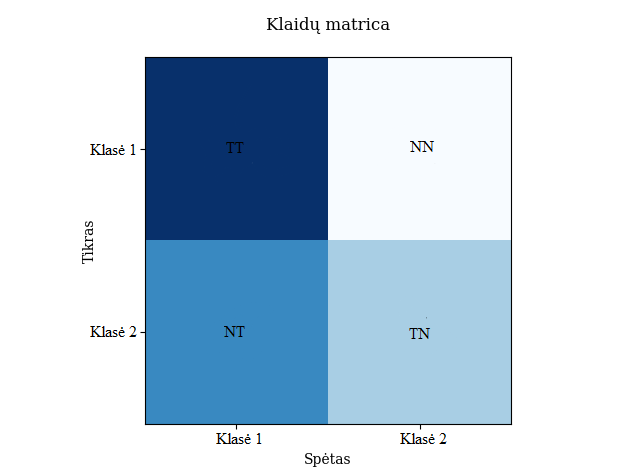
\includegraphics[width=0.6\textwidth]{img/KlaiduMatrica.png}
    \caption{Klaidų matricos pavyzdys}
    \label{fig:architecture}
\end{figure}
Taigi, jeigu modelis įvardina dalį klasės 1 paveiksliukų kaip klasę 1 tai tų paveiksliukų kiekis yra įrašomas į TT matricos laukelį. Tačiau jei modelis klasės 1 paveiksliukus įvardina kaip klasę 2, tai tas paveiksliukų skaičius yra įrašomas į NT laukelį. Tas pats vyksta su klasės 2 paveiksliukais, jeigu jie yra įvardinami kaip klasės 2 paveiksliukai, tas kiekis įrašomas į TN laukelį, tačiau jei kažkiek paveiksliukų įvardinama kaip klasės 1, tas skaičius įrašomas į NN laukelį. 

Pagal klaidų matricos duomenis galima apskaičiuoti kelias modelio metrikas - tikslumas, atšaukimas ir precizija.

\subsubsection{Tikslumas}
Tikslumas (angl. accuracy) yra matavimas, kuris parodo santykį tarp teisingai spėjimų (angl. prediction) ir iš viso darytų spėjimų.
\begin{equation}
\textit{tikslumas} = \frac{TT + TN}{TT + TN + NT + NN}.
\end{equation}

Formulės (3) parametras \(TT\) yra skaičius tikrų teigiamų spėjimų, \(TN\) yra skaičius tikrų neigiamų spėjimų ir \(NT\) yra skaičius netikrų teigiamų spėjimų bei \(NN\) yra skaičius netikrų neigiamų spėjimų.
Turinti pagal klases nesubalansuotą duomenų rinkinį (pvz. viena klasė turi daug daugiau duomenų negu likusios), tikslumo metrika nepilnai atskleidžia modelio gerumą. Pavyzdžiui, kačių nuotraukų yra 9, o šunų yra 91, modelis teisingai atpažįsta 1 katę ir 90 šunų, tikslumas bus 0.91, nors tik viena katė buvo atpažinta. 

\subsubsection{Atšaukimas}
Atšaukimas (angl. recall) yra metrika, kuri parodo santykį tarp visų teisingai atpažintų spėjimų ir visų esamų teigiamų spėjimų.
\begin{equation}
\textit{atšaukimas} = \frac{TT}{TT + NN}.
\end{equation}

Formulės (4) parametras \(TT\) yra skaičius tikrų teigiamų spėjimų, o \(NN\) yra skaičius netikrų neigiamų spėjimų. Sudėjus \(TT\) ir \(NN\) yra gaunama visos teigiamos reikšmės.
Aukštas atšaukimas parodo, kad klasė buvo teisingai atpažinta (mažas \(NN\)).

\subsubsection{Precizija}
Precizija (angl. precision) parodo kiek iš visų teigiamų spėjimų, jų buvo iš tiesų teisingi. 
\begin{equation}
\textit{precizija} = \frac{TT}{TT + NT}.
\end{equation}
Formulės (5) parametras \(TT\) yra skaičius tikrų teigiamų spėjimų, o \(NT\) yra skaičius netikrų teigiamų spėjimų. Sudėjus \(TT\) ir \(NT\) yra gaunama visi daryti teigiami spėjimai.
Aukšta precizija reiškia, kad reikšmė įvardinta kaip teigiama iš ties yra teigiama (mažas \(NT\)).

\section{Technologijos}
Naudojamų technologijų išsirinkimas yra pradinis žingsnis siekiant įvykdyti bakalauro darbe išsikeltas užduotis. Šiame skyriuje pateiktos populiariausios šių laikų technologijos 
bei glaustai apibrėžti jų pagrindiniai funkcionalumai.

\subsection{ImageNet}
Projektas ImageNet buvo sugalvotas profesorės Li Fei-Fei 2009 metais. Projekto tikslas buvo sukurti didelę sukategorizuotų paveiksliukų ir jų etikečių duomenų bazę, 
kuri butų skirta vizualinio objekto atpažinimo programinės įrangos tyrimams. Ši duomenų bazė yra suorganizuota pagal WorldNet hierarchija - anglų kalbos žodžiai 
yra grupuojami į sinonimų rinkinius, kurie turi apibūdinimus ir naudojimo pavyzdžius bei saugo ryšių kiekį tarp sinonimų arba jų narių. ImageNet turi daugiau nei 
100 000 sinonimų rinkinių, kur didžioji dalis yra daiktavardžiai (80 000+). 

ImageNet projektas kiekvienais metais daro konkursą vadinamą „ImageNet Large Scale Visual Recognition Challenge“ (trumpinys ILSVRC). Konkurso užduotis yra 
išmokinti modelį, kuris galėtų įvesties paveiksliuką teisingai klasifikuoti į 1000 skirtingų objektų klasių, kurios atitinka realius daiktus, gyvūnus ir t.t. Modeliai 
yra apmokomi su apie 1.2 milijonų paveiksliukų ir dar 50 000 paveiksliukų yra naudojami validacijai mokymo metu bei 100 000 paveiksliukų yra panaudojami galutiniam 
modelio testavimui. Šis konkursas yra paveiksliukų klasifikacijos algoritmų etalonas.

\subsection{Keras}
Keras yra aukšto lygio programų sąsaja skirta neuroniniams tinklams. Sąsaja parašyta su Python programavimo kalba ir vidinėje pusėje galinti veikti su „TensorFlow“ 
ir kitomis bibliotekomis. Keras buvo sukurtas tikintis suteikti greitą eksperimentavimą, kad sugalvojus idėją pasiekti rezultato būtų galima su kiek įmanoma mažiau uždelsimo.

Ši sąsaja savyje turi visus pagrindinius neuroninio tinklo kūrimo blokus, pavyzdžiui, sluoksniai, aktyvavimo ir optimizavimo funkcijos. Taip pat Keras suteikia modelius, 
kurie yra apmokyti naudojant ImageNet duomenų bazę. Šiuos modelius galima derinti, pridėti papildomų sluoksnių, pasirinkti esamus sluoksnius bei juos iš naujo apmokyti.

\subsection{TensorFlow}
TensorFlow yra atviros programinės įrangos biblioteka skirta aukšto našumo skaitiniams skaičiavimams. Jo lanksti architektūra leidžia lengvai diegti skaičiavimus įvairiose 
platformose - procesoriuose, grafikos procesoriuose. Sukurtas „Google“ dirbtinio intelekto skyriaus, tad yra labai palaikomas automatinis ir gilusis mokymasis, tačiau 
dėl bibliotekos ir skaičiavimų lankstumo yra naudojamas įvairiose mokslinėse srityse.

\section{Modelių derinimas su mažu duomenų rinkiniu} 
Šio eksperimento tikslas yra išanalizuoti skirtingų gylių neuroninius tinklus pagal metrikas gautas po mokymo ir validavimo naudojant mažą duomenų rinkinį. 
Poskyriuje „Architektūros“ yra trumpai apibūdinti pagrindiniai konvoliucinių neuroninių tinklų tipai. 
Iš jų buvo išsirinktas NASNet, kadangi jis yra inovatoriškiausias ir geriausią tikslumą turintis. Negilusis modelis buvo NASNetMobile, o gilusis - NASNetLarge.

Nuspręsta daryti paprastą binarinę paveikslėlių klasifikaciją.
Buvo surastos ir naudotos dvi skirtingos duomenų imtys - kačių ir šunų bei virtuvės ir gyvenamojo kambario. Jos abi turėjo 1400 paveikslėlių - 1 300 mokymosi tikslui ir 100 validacijos.

\subsection{Tinklelio paieška}

Taikant paieškos strategiją - tinklelio paiešką - buvo ieškoma geriausių hiperparametrų NASNetMobile ir NASNetLarge modeliams su dviem skirtingais duomenų rinkiniais ir keičiant mokomų sluoksnių skaičių.

Pagal naudojamo kompiuterio pajėgumą buvo nuspręsta tyrinėti:
\begin{itemize}
    \item Išmetimo sluoksnio reikšmę - 0.25, 0.5 ir 0,75.
    \item Optimizavimo funkciją - RMSprop, Adam, Adagrad.
    \item Mokymosi greitį - 0.0005, 0.0001 ir 0.001.
    \item Mokomų sluoksnių skaičius - 5, 10, 20.
\end{itemize}

Iš visų šių hiperparametrų susidarė 27 kombinacijos bei jos buvo analizuojamos 12 kartų - su NASNetMobile ir dviem skirtingais duomenų rinkiniais bei keičiant mokomų sluoksnių skaičių, su NASNetLarge ir tais pačiais duomenų rinkiniais bei keičiant mokomų sluoksnių skaičių.
Pagrindinis rezultatų rikiavimo kriterijus buvo tikslumas, antrinis - atšaukimas, o paskutinis buvo precizija. Visi rezultatai pateikti Prieduose esančioje 3 lentelėje. 
Pagal gautus rezultatus buvo nuspręsta išmetimo sluoksnio reikšmę nustatyti 0.25, optimizavimo funkciją kaip Adagrad su 0.0001 mokymosi greičiu.


\subsection{Programos veikimas}
Ankstesniame skyriuje „Technologijos“ yra išvardintos visos technologijos, kurios buvo naudotos šiam eksperimentui.

Eksperimentui įvykdyti reikėjo paruošti kompiuterį darbui - įrašyti „Python“ programavimo įrankius, paruošti „Anaconda“ komandinę eilutę, „NVIDIA CUDA“ įrankius, Keras ir 
TensorFlow. Naudojamas kompiuteris privalo turėti galingą procesorių ar grafinį procesoriaus bloką - kompiuteris, kuris buvo naudotas eksperimentui, turėjo Nvidia 1080 Ti. 
 
Keras pateikia modelius, apmokytus su ImageNet, ir jų svorius, todėl reikėjo importuoti 
tinkamą modelį - šiuo atveju NASNet. Importavimo metu padaryti nustatymai - pilnai sujungtas sluoksnis nepridedamas, kadangi tada galima parinkti kokių dimensijų 
paveiksliukai naudojami ir kiek spalvų sluoksnių jie turi (standartiniai paveiksliukai turi 3). Tuomet reikėjo nustatyti kiek importuoto modelio sluoksnių bus mokoma norima - 5, 10 ir 20. 
Po šių egzistuojančio modelio paruošimų reikėjo sukurti naują Kero modelį, prie kurio reikėjo pridėti paruoštą egzistuojantį modelį bei pridėti kelis kitus sluoksnius tam tikru išsidėstymu - 
plokštinimo (angl. flatten), tankumo (angl. dense), išmetimo (angl. dropout) ir vėl tankumo. Pirmasis tankumo sluoksnis turi aktyvacijos funkciją ReLU, o paskutinis - sigmoidinę. 
Po visų sluoksnių pridėjimo negilus modelis iš viso turėjo 4 405 141 parametrų, o gilusis modelis turėjo 85 916 818.

Po modelio paruošimo, reikėjo nustatyti kokio dydžio paveikslėlių partijomis (angl. batch) bus mokomas ir validuojamas modelis. Geriausias partijos dydis naudotam kompiuteriui buvo mokymosi partijai 130 paveikslėlių, o validacijos - 10.
Tuomet nustatomas paveikslėlių aplankalo kelias, jų ir partijos dydis bei nustatomas klasės režimas į binarinį, nes duomenų imtis susideda iš dviejų klasių - kačių ir šunų arba virtuvės ir gyvenamojo kambario.

Po modelio ir paveikslėlių rinkinio paruošimo buvo pradėta mokinti ir validuoti modelį. Taigi, modelio kompiliavimo metode nuostolio 
funkcija buvo nustatyta binarine kryžiaus entropija, o optimizavimo funkcija - Adagrad. Po modelio sukompiliavimo buvo paleidžiamas mokymo metodas, kuriam turi būti pateikta - paruošti paveiksliukai, žingsnis per epochą, epochų kiekis, 
paruošti validacijos paveiksliukai ir jų žingsnis. Epochų kiekis šiame eksperimente buvo nustatyta 5.

\subsection{Modelių derinimas}
Buvo pradėta derinti ir validuoti modelius su skirtingais duomenų rinkiniais ir keičiant mokomų sluoksnių skaičių.

\subsubsection{Negilaus modelio derinimas}
Eksperimentas buvo pradėtas nuo negilaus modelio (NASNetMobile) derinimo.

NASNetMobile modelis buvo derinamas su gyvūnų (kačių ir šunų) duomenų rinkiniu ir mokomų sluoksnių skaičiumus buvo nustatytas 5-iems.
Po derinimo buvo gauti tikslumo ir nuostolio grafai - 15 ir 16 pav. (Priedas nr. 2). Iš jų matyti kad mokymo tikslumas tiesiškai augo, o nuostolis tiesiškai mažėjo, tačiau validacijos tikslumas nuo 0.5 pakilo tik 0.5 ir nuostolis išliko autkštas.

Po to modelis buvo derinamas su kambarių (virtuvės ir svetainės) duomenų rinkiniu bei tokiu pačių mokomų sluoksnių skaičiumi.
Gauti rezultatai pateikti 17 ir 18 pav. (Priedas nr. 2). Mokymo ir validavijos tikslumas nepasiekė tokio tikslumo kaip kad modelį derinant su gyvūnų rinkiniu, nors ir mokymo tikslumas nuolatos didėjo, validacijos tikslumas svyravo ir paskutinėje epochoje pasiekė mažiausias reikšmes. Tačiau nuostolio grafikas parodo tokias pačias tendencijas kaip kad derinant su gyvūnų rinkiniu.

Taigi, iš gautų klaidų matricų (3 ir 4 pav.) galima matyti, jog derinant modelį su gyvūnų rinkiniu buvo geriau nustatytos klasės. 
Su gyvūnų rinkiniu buvo pasiektas tikslumas - 0.57, atšaukimas - 0.94, precizija - 0.54, kai su kambarių rinkiniu buvo gautas tikslumas - 0.53, atšaukimas - 0.74, precizija - 0.52.
\begin{figure}[!htbp]
    \centering
    \begin{minipage}[b]{0.48\textwidth}
      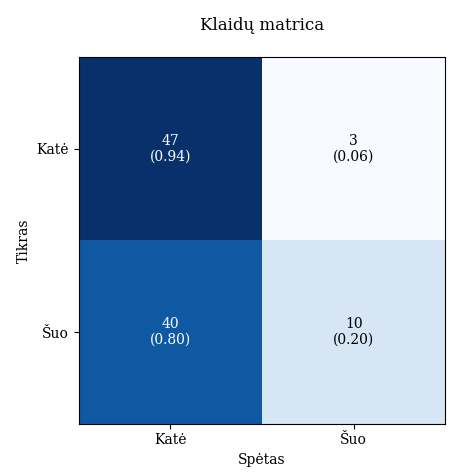
\includegraphics[width=\textwidth]{img/GrapthsNEW/Small/animal/5/KM_DC_S_5.png}
      \caption{Klaidų matrica gauta su gyvūnų duomenų rinkiniu}
    \end{minipage}
    \hspace{2mm}
    \begin{minipage}[b]{0.48\textwidth}
      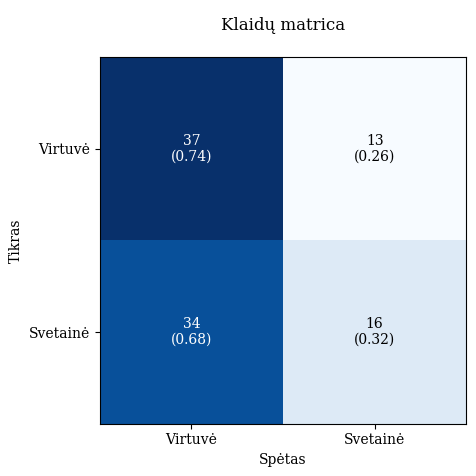
\includegraphics[width=\textwidth]{img/GrapthsNEW/Small/room/5/KM_R_S_5.png}
      \caption{Klaidų matrica gauta su kambarių duomenų rinkiniu}
    \end{minipage}
\end{figure}

Iš naujo buvo derinamas negilus modelis su gyvūnų rinkiniu ir su 10 mokomų sluoksnių. 
Po derinimo gauti rezultatai pateikti 19 ir 20 pav. (Priedas nr. 2). Mokymo tikslumas nuolatos didėjo, o validacijos svyravo, tačiau paskutinėse epochose išsitiesino. O mokymo ir validacijos nuostolis nuolatos mažėjo.

Modelis buvo derinamas su tokiu pačiu mokomų sluoksnių skaičiumi, bet su kambarių duomenų rinkiniu.
Gauti rezultatai pateikti 21 ir 22 pav. (Priedas nr. 2). Mokymo tikslumas visą laiką buvo mažesnis negu validacijos, tačiau paskutinėje epochoje tikslumai pasiekė tokią pačią reikšmę. O mokymo nuostolis nuolatos mažėjo ir po paskutinės epochos buvo mažesnis už validacijos. 

Po šių derinimų buvo gautos klaidų matricos - 5 ir 6 pav. Su tokiu mokomų sluoksnių skaičiumi modelis derinamas su kambarių rinkiniu teisingai atpažino daugiau klasių negu kad modelis su gyvūnų rinkiniu. 
Su gyvūnų rinkiniu buvo pasiektas tikslumas - 0.52, atšaukimas - 0.28, precizija - 0.54, kai su kambarių rinkiniu buvo gautas tikslumas - 0.55, atšaukimas - 0.80, precizija - 0.53.

\begin{figure}[!htbp]
    \centering
    \begin{minipage}[b]{0.48\textwidth}
      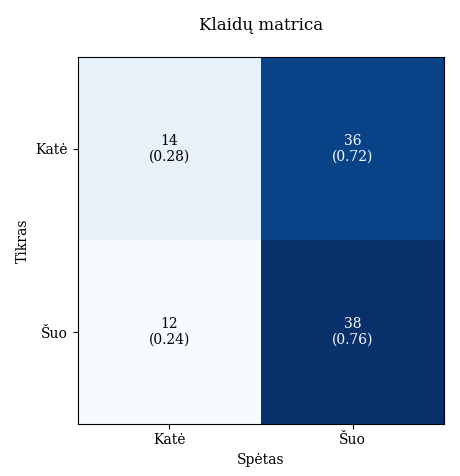
\includegraphics[width=\textwidth]{img/GrapthsNEW/Small/animal/10/KM_DC_S_10.png}
      \caption{Klaidų matrica gauta su gyvūnų duomenų rinkiniu}
    \end{minipage}
    \hspace{2mm}
    \begin{minipage}[b]{0.48\textwidth}
      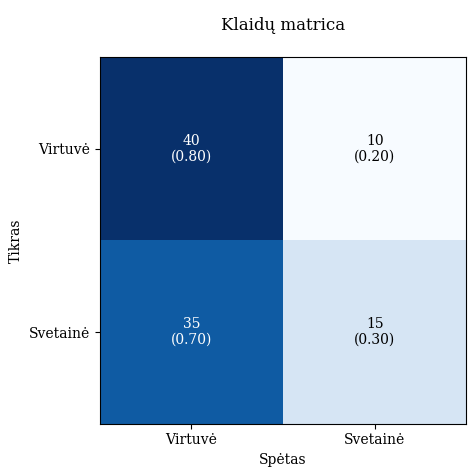
\includegraphics[width=\textwidth]{img/GrapthsNEW/Small/room/10/KM_R_S_10.png}
      \caption{Klaidų matrica gauta su kambarių duomenų rinkiniu}
    \end{minipage}
\end{figure}

Negilaus modelio derinimas buvo daromas su 20 mokomų sluoksnių ir gyvūnų duomenų rinkiniu.
Po derinimo buvo gauti tikslumo ir nuostolio grafai - 23 ir 24 pav. (Priedas nr. 2). Juose pateikta kad mokymo ir validacijos tikslumas kilo, nors validacijos tikslumas 2-oje epochoje buvo sumažėjęs. O nuostolio grafikai pateikta kad mokymo ir validacijos reikšmės nuolatos mažėjo, tačiau mokymo nuostolis mažėjo daug greičiau.

Paskutinis NASNetMobile modelio derinimas buvo daromas su kambarių duomenų rinkiniu ir tokiu pačiu mokomų sluoksnių skaičiumi kaip kad su gyvūnų rinkiniu. 
Gauti rezultatai pateikti 25 ir 26 pav. (Priedas nr. 2). Juose yra pateikta jog mokymo ir validacijos tikslumas nuolatos didėjo, o nuostolis mažėjo nors validacijos tikslumas ir nuostolis daug plokščiau negu kad mokymosi tikslumas ir nuostolis.

Po paskutinių negilaus modelio derinimų buvo gautos klaidų matricos, kurios pateiktos 7 ir 8 pav. Jose parodyta jog modelis derintas su gyvūnų duomenų rinkiniu pranoko modelį derintą su kambarių duomenų rinkiniu.
Su gyvūnų rinkiniu buvo pasiektas tikslumas - 0.69, atšaukimas - 1.00, precizija - 0.62, kai su kambarių rinkiniu buvo gautas tikslumas - 0.61, atšaukimas - 0.88, precizija - 0.57.

\begin{figure}[!htbp]
    \centering
    \begin{minipage}[b]{0.48\textwidth}
      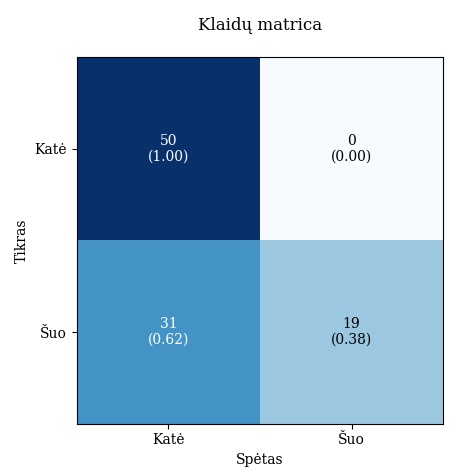
\includegraphics[width=\textwidth]{img/GrapthsNEW/Small/animal/20/KM_DC_S_20.png}
      \caption{Klaidų matrica gauta su gyvūnų duomenų rinkiniu}
    \end{minipage}
    \hspace{2mm}
    \begin{minipage}[b]{0.48\textwidth}
      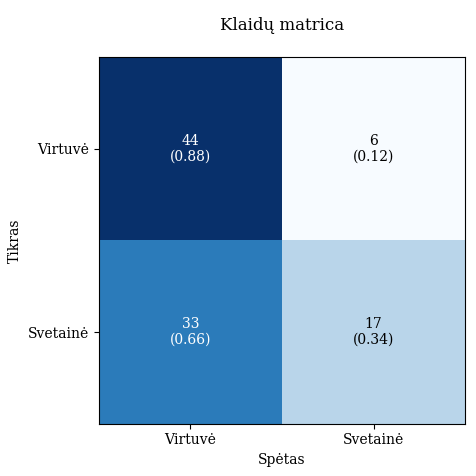
\includegraphics[width=\textwidth]{img/GrapthsNEW/Small/room/20/KM_R_S_20.png}
      \caption{Klaidų matrica gauta su kambarių duomenų rinkiniu}
    \end{minipage}
\end{figure}

Taigi, derinant negilų modelį su gyvūnų arba kambarių duomenų rinkiniais aukščiausias tikslumas, atšaukimas ir precizija buvo pasiekti mokomų sluoksnių skaičių nustačius 20. Tačiau modeliai, kurie buvo suderinti su gyvūnų duomenų rinkiniu, dažniau pasiekė aukštesnius rezultatus negu modeliai, kurie buvo suderinti su kambarių rinkiniu. 
%--------------------------------------------------------------------------------------------

\subsubsection{Gilaus modelio derinimas}
Eksperimentas buvo pratęstas naudojant gilų modelį (NASNetLarge).

Gilų modelį derinti buvo pradėta su gyvūnų duomenų rinkiu ir 5-iais mokomais sluoksniais.
Gauti rezultatai pateikti 27 ir 28 pav. (Priedas nr. 2). Modelio mokymo tiklsumas augo logaritmiškai, o validacijos tikslumas nuolatos plokščiai mažėjo. Nors mokymo ir validacijos nuostoliai panašiai nuolatos mažėjo.

Po to gilus modelis buvo apmokytas su kambarių duomenų rinkiniu ir 5-iais mokomais sluoksniais.
Po derinimo buvo gauti tikslumo ir nuostolio grafai - 29 ir 30 pav. (Priedas nr. 2). Juose pateikta kad validacijos tikslumas šiek tiek svyravo, bet nuolatos augo ir buvo didesnis už mokymo tikslumą. O mokymo ir validacijos nuostoliai nuolatos panašiai mažėjo.

Po derinimų buvo gautos klaidų matricos, kurios pateiktos 9 ir 10 pav. Jose parodyta, jog modelis suderintas su gyvūnų duomenų rinkiniu atpažino šiek tiek daugiau klasių negu kad modelis apmokytas su kambarių duomenų rinkiniu.
Su gyvūnų rinkiniu buvo pasiektas tikslumas - 0.92, atšaukimas - 0.98, precizija - 0.88, kai su kambarių rinkiniu buvo gautas tikslumas - 0.87, atšaukimas - 0.86, precizija - 0.88.

\begin{figure}[!htbp]
    \centering
    \begin{minipage}[b]{0.48\textwidth}
      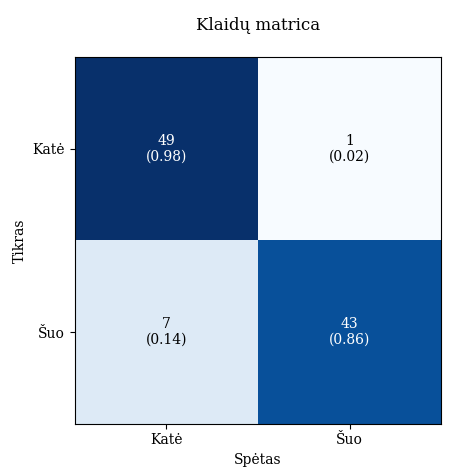
\includegraphics[width=\textwidth]{img/GrapthsNEW/Large/animal/5/KM_DC_L_5.png}
      \caption{Klaidų matrica gauta su gyvūnų duomenų rinkiniu}
    \end{minipage}
    \hspace{2mm}
    \begin{minipage}[b]{0.48\textwidth}
      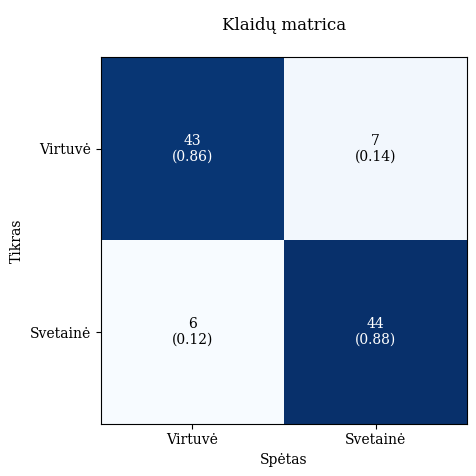
\includegraphics[width=\textwidth]{img/GrapthsNEW/Large/room/5/KM_R_L_5.png}
      \caption{Klaidų matrica gauta su kambarių duomenų rinkiniu}
    \end{minipage}
\end{figure}

NASNetLarge buvo derinamas su gyvūnų duomenų rinkiniu ir mokomų sluoksnių skaičiumus buvo nustatytas 10.
Gauti rezultatai pateikti 31 ir 32 pav. (Priedas nr. 2). Juose pateikta jog mokymo ir validacijos tikslumas auga, tačiau paskutinėse keliose epochose pradeda mažėti. O mokymo ir validacijos nuostoliai nuolatos mažėja.

Modelis iš naujo derinamas su kambarių duomenų rinkiniu ir tokiu pačiu mokomų sluoksnių skaičiumi kaip kad su gyvūnų rinkiniu.
Po derinimo buvo gauti grafikai - 33 ir 34 pav. (Priedas nr. 2). Mokymo ir validacijos tikslumas nuolatos didėjo, tačiau validacijos tikslumas buvo nuolatos didesnis už mokymo. Nors mokymo ir validacijos nuostoliai nuolatos mažėja.

Po padarytų modelių derinimų buvo gautos klaidų matricos - 11 ir 12 pav., kuriose pateikta jog modelis, kuris buvo derinamas su gyvūnų rinkiniu, teisingai atpažino daugiau klasių.
Su gyvūnų rinkiniu buvo pasiektas tikslumas - 0.93, atšaukimas - 1.00, precizija - 0.88, kai su kambarių rinkiniu buvo gautas tikslumas - 0.91, atšaukimas - 0.92, precizija - 0.90.

\begin{figure}[!htbp]
    \centering
    \begin{minipage}[b]{0.48\textwidth}
      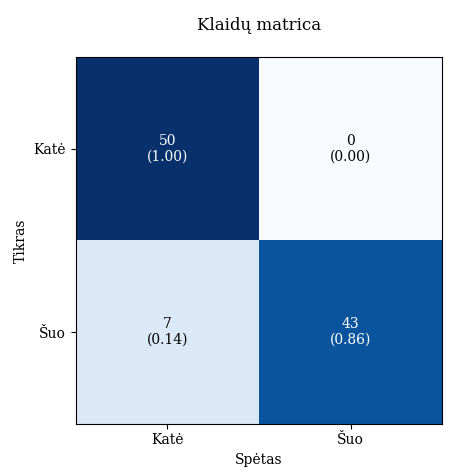
\includegraphics[width=\textwidth]{img/GrapthsNEW/Large/animal/10/KM_DC_L_10.png}
      \caption{Klaidų matrica gauta su gyvūnų duomenų rinkiniu}
    \end{minipage}
    \hspace{2mm}
    \begin{minipage}[b]{0.48\textwidth}
      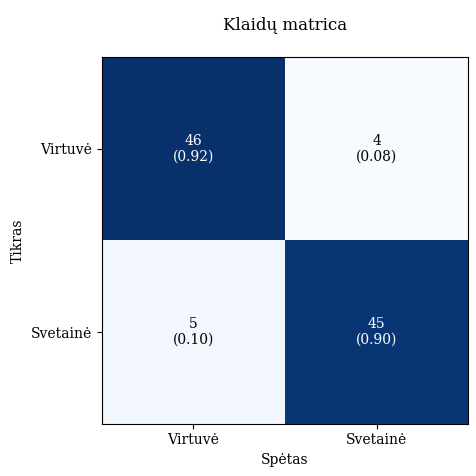
\includegraphics[width=\textwidth]{img/GrapthsNEW/Large/room/10/KM_R_L_10.png}
      \caption{Klaidų matrica gauta su kambarių duomenų rinkiniu}
    \end{minipage}
\end{figure}


Gilus modelis buvo derinamas su gyvūnų duomenų rinkiniu ir mokomų sluoksnių skaičius buvo nustatytas 20.
Po derinimo buvo gauti grafikai - 35 ir 36 pav. (Priedas nr. 2). Juose pateikta jog modelio mokymo tikslumas nuolatos augo, o validacijos tikslumas šiek tiek svyravo. O mokymo ir validacijos nuostoliai nuolatos mažėja.

Paskutiniame NASNetLarge modelio derinime buvo naudotas kambarių duomenų rinkinys ir 20-imt mokomų sluoksnių.
Gauti rezultatai pateikti 37 ir 38 pav. (Priedas nr. 2). Juose parodyta kad mokymo ir validacijos tikslumas nuolatos augo, tačiau tikslumas prieš paskutinėje epochoje pradėjo mažėti. Nors mokymo ir validacijos nuostoliai nuolatos mažėja.

Po paskutinių modelio derinimų gautos klaidų matricos, kurios pateiktos 13 ir 14 pav., kuriose pateikta jog modelis suderintas su gyvūnų duomenų rinkiniu teisingai atpažino daugiau klasių negu kad kitas modelis.
Su gyvūnų rinkiniu buvo pasiektas tikslumas - 0.96, atšaukimas - 1.00, precizija - 0.93, kai su kambarių rinkiniu buvo gautas tikslumas - 0.89, atšaukimas - 0.92, precizija - 0.87.

\begin{figure}[!htbp]
    \centering
    \begin{minipage}[b]{0.48\textwidth}
      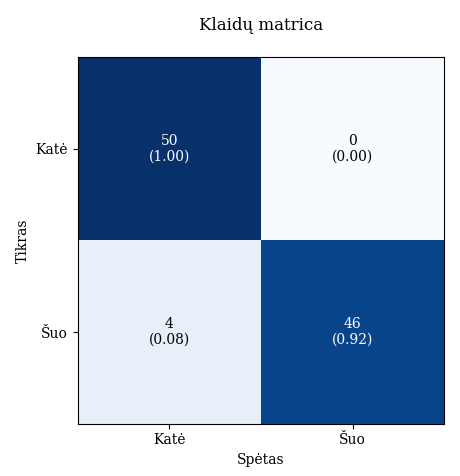
\includegraphics[width=\textwidth]{img/GrapthsNEW/Large/animal/20/KM_DC_L_20.png}
      \caption{Klaidų matrica gauta su gyvūnų duomenų rinkiniu}
    \end{minipage}
    \hspace{2mm}
    \begin{minipage}[b]{0.48\textwidth}
      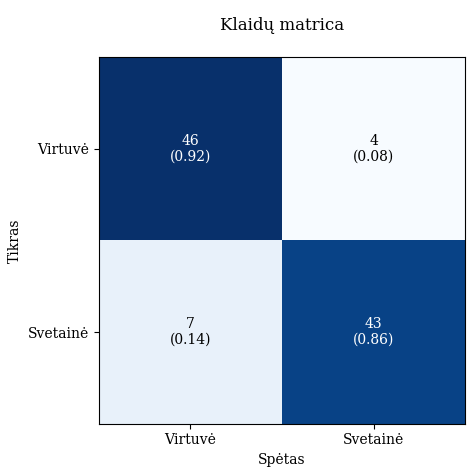
\includegraphics[width=\textwidth]{img/GrapthsNEW/Large/room/20/KM_R_L_20.png}
      \caption{Klaidų matrica gauta su kambarių duomenų rinkiniu}
    \end{minipage}
\end{figure}

Taigi, geriausius rezultus modelis suderintas su gyvūnų duomenų rinkiniu pasiekia naudojant 20 mokomų sluoksnių, o modelis suderintas su kambarių duomenų rinkiniu pasiekia aukščiausius rezultatus mokomų sluoksnių skaičių nustačius 10.

\sectionnonum{Rezultatai}
Šio darbo metu buvo tirta dirbtinių neuroninių tinklų ir konvoliucinių neuroninių tinklų veikimas 
ir jų sudedamosios dalys bei surinkta informacija iš litertūros šaltinių. Atliktas eksperimentas, 
kurio tikslas buvo pamatyti kokį poveikį turi konvoliucinio neuroninio tinklo gylis ir jo suderinimui 
naudojamas mažas duomenų rinkinys neuroninio tinklo metrikoms - tikslumui, atšaukimui, precizijai.

Darbo rezultatai:
\begin{enumerate}
    \item Buvo atlikta bendra dirbtinių neuroninių tinklų ir konvoliucinių neuroninių tinklų bei NAS algoritmo analizė.
    \item Buvo rasti geriausi hiperparametrai (optimizavimo funkcija, mokymosi greitis, išmetimo sluoksnio reikšmė) NASNetLarge ir NASNetMobile modeliams naudojant du skirtingus duomenų rinkinius bei keičiant mokomų sluoknsių skaičių.
    \item Egzistuojantys NASNetLarge ir NASNetMobile modeliai buvo modifikuoti binariniai klasifikacijai ir suderinti naudojant du skirtingus duomenų rinkinius - kačių ir šunų bei virtuvės ir gyvenamojo kambario.
    \item Gauti skirtingų gylių suderintų modelių mokymo ir validacijos tikslumo grafikai bei klaidų matricos.
\end{enumerate}

\sectionnonum{Išvados}
Atlikus litertūros šaltinių analizę ir eksperimentą buvo padarytos išvados:
\begin{enumerate}
  \item Suderinus skirtingų gylių modelius su dviem skirtingais mažais duomenų rinkiniais ir keičiant mokomų sluoksnių skaičių, buvo nustatyta, kad gilesnis tinklas pasiekė daug aukštesnius rezultatus (tikslumą, atšaukimą, preciziją) negu negilus modelis. Gilaus modelio validacijos tikslumo vidurkis buvo 0.91, atšaukimo vidurkis buvo 0.95 ir precizijos buvo 0.89, kai su tokiais pačiais hiperparametrais ir duomenų rinkiniais negilaus modelio validacijos tikslumo vidurkis buvo 0.58, atšaukimo vidurkis buvo 0.77 bei precizijos vidurkis buvo 0.55. Taigi, šio eksperimento metu gilesnis tinklas pasiekė 58\% didesnį tikslumą, 22\% didesnį atšaukimą ir 60\% didesnią preziją palyginus su negilaus modelio rezultatais.
  \item Modelis, kuris buvo pirmiausia apmokytas su duomenų rinkiniu, kuriame egzistuoja klasės sutampančios su derinimui naudojamu duomenų rinkinio klasėmis, po suderinimo gaus šiek tiek geresnius rezultatus negu kad toks pat modelis, kuris buvo suderintas su duomenų rinkiniu, kurio klasės nesutampa. Tai buvo nustatyta, kadangi naudojami modeliai buvo apmokyti su ImageNet duomenų baze, kurioje egzistuoja kačių ir šunų klasės, o derinant šiuos modelius su kačių ir šunų duomenų rinkiniais buvo gautas validacijos tikslumo vidurkis 0.77, atšaukimo vidurkis buvo 0.87 bei precizijos vidurkis buvo 0.73, o modelių suderintų su virtuvės ir svetainės duomenų rinkiniu validacijos tikslumo vidurkis buvo 0.73, atšaukimo vidurkis buvo 0.85, o precizijos vidurkis buvo 0.71. Taigi, suderintas modelis su duomenų rinkiniu, kurio klasės yra žinomos modeliui, pasiekia 5\% didesnį tikslumą, 1\% didesnį atšaukimą ir 2\% didesnią preciziją negu suderintas modelis su duomenų rinkiniu, kurio klasės yra naujos modeliui.
  \item Mokomų sluoksnių skaičius buvo keičiamas derinant skirtingų gylių modelius su dviem skirtingais mažais duomenų rinkiniais. Buvo pasirinkti sluoksnių skaičiai - 5, 10 ir 20. Palyginus visus bandymus geriausi rezultatai buvo pasiekti mokomų sluoksnių skaičių nustačius 20, tačiau derinant gilesnį modelį su virtuvės ir svetainės duomenų rinkiniu geriausias rezultatas buvo pasiektas su 10 mokomų sluoksnių. Su 5-iais mokomais sluoksniais modelis turėjo 0.72 tikslumo vidurkį, 0.88 atšaukimo vidurkį ir 0.71 precizijos vidurkį, su 10-imt mokomų sluoksnių modelio tikslumo vidurkis buvo 0.73, atšaukimo vidurkis buvo 0.75 bei precizijos vidurkis buvo 0.71. Tačiau su 20-imt mokomų sluoksnių modelis turėjo 0.79 tikslumo vidurkį, 0.95 atšaukimo vidurkį ir 0.75 precizijos vidurkį. Taigi, nustačius mokomų sluoksnių skaičių kaip 20 buvo pasiekti geresni rezultatai.
\end{enumerate}



\printbibliography[heading=bibintoc]

% \sectionnonum{Sąvokų apibrėžimai ir santrumpos}
% AutoML - (angl. automated machine learning) automatizuotas mašininis mokymasis.

% Hiperparametrai - (angl. hyperparameters) vidiniai neuroninio tinklo parametrai.

% Derinimas - (angl. fine-tune) apmokyto modelio dalinis mokymas su kitu duomenų rinkiniu.

% Pagreitis - (angl. momentum) dydis, kuris pirmiausiai leidžia greičiau judėti tam kad peršokti lokalius minimumus. Tačiau artėjant link konvergavimo šis dydis mažėja tam kad nebūtų praleistas globalus minimumas. 

\appendix
\section{Tinklelio paieška}
Hiperparametrų stulpelyje yra pateiktos išmetimo sluoksnio, optimizacijos funkcijos, mokymosi greičio reikšmės. Jų tyrinėjimas buvo atliktas su NASNetLarge ir NASNetMobile modeliais naudojant gyvūnų (kačių ir šunų) ir kambarių (virtuvės ir gyvenamojo kambario) duomenų rinkinius bei keičiant mokomų sluoksnių skaičių (5, 10 ir 20). Kiekviename rezultatų langelyje pateiktos tikslumo, atšaukimo ir precizijos reikšmės. Paryškintos reikšmės parodo geriausius rezultatus tame stulpelyje. 
\setlength\LTleft{-0.8in}
\setlength\LTright{-1in}
\begin{longtable}{ | p{1.5cm} | p{1cm} | p{1cm} | p{1cm} | p{1cm} | p{1cm} | p{1cm} | p{1cm} | p{1cm} | p{1cm} | p{1cm} | p{1cm} | p{1cm} | }
    \caption{Rezultatai} \\
    \hline
    \multirow{3}{1.5cm}{Hiperpara- metrai} & \multicolumn{6}{c|}{NASNetLarge} & \multicolumn{6}{c|}{NASNetMobile} \\ \cline{2-13}
    & \multicolumn{3}{|c}{Gyvūnai} & \multicolumn{3}{|c}{Kambariai} & \multicolumn{3}{|c}{Gyvūnai} & \multicolumn{3}{|c|}{Kambariai} \\ \cline{2-13}
    & 5 & 10 & 20 & 5 & 10 & 20 & 5 & 10 & 20 & 5 & 10 & 20 \\  \hline
    \endhead
    0.25, RMSprop, 0.0005 & 0.96; 0.94; 0.98 & 0.89; 0.78; 1.0 & 0.96; 0.92; 1.0  &  0.89; 0.84; 0.93 & 0.88; 0.8; 0.95 & 0.86; 0.74; 0.97   &  0.67; 0.34; 1.0 & 0.69; 0.38; 1.0 & 0.58; 0.16; 1.0             &  0.5; 0.0; 0.0 & 0.53; 0.06; 1.0 & 0.54; 0.08; 1.0  \\ \hline
    0.25, RMSprop, 0.0001 & 0.92; 0.84; 1.0 & 0.95; 0.9; 1.0 & \textbf{0.98; 0.96; 1.0}    &  0.88; 0.84; 0.91 & \textbf{0.91; 0.88; 0.94} & 0.88; 0.82; 0.93  &  0.6; 0.2; 1.0 & 0.7; 0.44; 0.92 & 0.61; 0.22; 1.0  &  0.51; 0.02; 1.0 & 0.58; 0.24; 0.75 & 0.58; 0.16; 1.0  \\ \hline
    0.25, RMSprop, 0.001  & 0.93; 0.86; 1.0 & 0.92; 0.84; 1.0 & 0.92; 0.84; 1.0   & 0.85; 0.72; 0.97 & 0.85; 0.86; 0.84 & \textbf{0.91; 0.9; 0.92}    &  0.63; 0.26; 1.0 & 0.62; 0.24; 1.0 & 0.58; 0.16; 1.0    &  0.5; 0.0; 0.0 & 0.5; 0.0; 0.0 & 0.66; 0.32; 1.0  \\ \hline
    0.25, Adam, 0.0005    & 0.91; 0.82; 1.0 & 0.91; 0.82; 1.0 & 0.93; 0.86; 1.0   &  0.89; 0.82; 0.95 & 0.88; 0.8; 0.95 & 0.89; 0.82; 0.95   &  0.56; 0.12; 1.0 & 0.67; 0.34; 1.0 & 0.62; 0.24; 1.0             &  0.5; 0.0; 0.0 & 0.5; 0.0; 0.0 & 0.52; 0.04; 1.0  \\ \hline
    0.25, Adam, 0.0001    & 0.95; 0.9; 1.0 & 0.94; 0.88; 1.0 & 0.93; 0.86; 1.0    &  0.88; 0.8; 0.95 & 0.9; 0.86; 0.93 & 0.89; 0.84; 0.93    &  0.62; 0.24; 1.0 & 0.69; 0.4; 0.95 & 0.61; 0.22; 1.0             &  0.54; 0.16; 0.67 & 0.48; 0.02; 0.25 & 0.51; 0.02; 1.0  \\ \hline
    0.25, Adam, 0.001     & 0.93; 0.86; 1.0 & 0.92; 0.84; 1.0 & 0.94; 0.88; 1.0   &  0.89; 0.82; 0.95 & 0.88; 0.8; 0.95 & 0.88; 0.8; 0.95    &  0.63; 0.26; 1.0 & 0.65; 0.3; 1.0 & 0.63; 0.26; 1.0              &  0.5; 0.0; 0.0 & 0.5; 0.0; 0.0 & 0.66; 0.32; 1.0  \\ \hline
    0.25, Adagrad, 0.0005 & 0.94; 0.88; 1.0 & 0.93; 0.86; 1.0 & 0.95; 0.9; 1.0    &  0.86; 0.78; 0.93 & 0.89; 0.84; 0.93 & 0.9; 0.86; 0.93   &  0.6; 0.2; 1.0 & 0.62; 0.24; 1.0 & 0.63; 0.26; 1.0               &  0.52; 0.04; 1.0 & 0.63; 0.36; 0.78 & 0.49; 0.0; 0.0  \\ \hline
    0.25, Adagrad, 0.0001 & \textbf{0.98; 0.96; 1.0} & 0.96; 0.92; 1.0 & 0.96; 0.92; 1.0   &  0.85; 0.78; 0.91 & 0.87; 0.94; 0.82 & 0.9; 0.88; 0.92   &  0.56; 0.18; 0.75 & 0.55; 0.1; 1.0 & 0.61; 0.22; 1.0    &  0.54; 0.4; 0.56 & \textbf{0.63; 0.56; 0.65} & 0.59; 0.26; 0.76  \\ \hline
    0.25, Adagrad, 0.001  & 0.93; 0.86; 1.0 & 0.92; 0.84; 1.0 & 0.96; 0.92; 1.0   &  0.88; 0.82; 0.93 & 0.85; 0.72; 0.97 & 0.88; 0.78; 0.97  &  0.67; 0.34; 1.0 & 0.65; 0.3; 1.0 & 0.67; 0.34; 1.0              &  0.5; 0.0; 0.0 & 0.52; 0.04; 1.0 & 0.52; 0.04; 1.0  \\ \hline
    0.5,  RMSprop, 0.0005  & 0.9; 0.8; 1.0 & 0.97; 0.94; 1.0 & 0.89; 0.78; 1.0     &  0.9; 0.82; 0.98 & 0.88; 0.86; 0.9 & 0.88; 0.78; 0.97   &  0.65; 0.3; 1.0 & 0.59; 0.18; 1.0 & 0.66; 0.32; 1.0              &  0.5; 0.0; 0.0 & 0.51; 0.02; 1.0 & 0.58; 0.16; 1.0  \\ \hline
    0.5,  RMSprop, 0.0001  & 0.95; 0.9; 1.0 & \textbf{0.98; 0.96; 1.0} & 0.95; 0.9; 1.0     &  0.89; 0.84; 0.93 & 0.9; 0.88; 0.92 & 0.88; 0.82; 0.93  &  0.58; 0.16; 1.0 & 0.59; 0.18; 1.0 & 0.72; 0.44; 1.0    &  0.55; 0.1; 1.0 & 0.54; 0.14; 0.7 & 0.52; 0.04; 1.0  \\ \hline
    0.5,  RMSprop, 0.001   & 0.95; 0.9; 1.0 & 0.89; 0.78; 1.0 & 0.93; 0.86; 1.0    &  0.88; 0.8; 0.95 & 0.89; 0.9; 0.88 & 0.85; 0.72; 0.97   &  0.63; 0.26; 1.0 & 0.55; 0.1; 1.0 & 0.62; 0.24; 1.0              &  0.5; 0.0; 0.0 & 0.52; 0.04; 1.0 & 0.57; 0.14; 1.0  \\ \hline
    0.5, Adam, 0.0005     & 0.91; 0.82; 1.0 & 0.91; 0.82; 1.0 & 0.95; 0.9; 1.0    &  0.86; 0.74; 0.97 & 0.88; 0.8; 0.95 & 0.89; 0.8; 0.98    &  0.63; 0.26; 1.0 & 0.68; 0.4; 0.91 & 0.67; 0.34; 1.0    &  0.51; 0.02; 1.0 & 0.51; 0.02; 1.0 & 0.52; 0.04; 1.0  \\ \hline
    0.5, Adam, 0.0001     & 0.95; 0.9; 1.0 & 0.93; 0.86; 1.0 & 0.93; 0.86; 1.0    &  0.89; 0.84; 0.93 & 0.89; 0.82; 0.95 & 0.88; 0.82; 0.93  &  \textbf{0.76; 0.54; 0.96} & 0.6; 0.2; 1.0 & 0.65; 0.3; 1.0      &  0.63; 0.3; 0.88 & 0.54; 0.16; 0.67 & 0.52; 0.04; 1.0  \\ \hline
    0.5, Adam, 0.001      & 0.88; 0.76; 1.0 & 0.93; 0.86; 1.0 & 0.95; 0.9; 1.0    &  0.86; 0.74; 0.97 & 0.86; 0.74; 0.97 & 0.88; 0.78; 0.97  &  0.55; 0.1; 1.0 & 0.65; 0.3; 1.0 & 0.61; 0.22; 1.0               &  0.5; 0.0; 0.0 & 0.51; 0.02; 1.0 & 0.63; 0.26; 1.0  \\ \hline
    0.5, Adagrad, 0.0005  & 0.93; 0.86; 1.0 & 0.94; 0.88; 1.0 & 0.95; 0.9; 1.0    &  0.88; 0.84; 0.91 & 0.89; 0.82; 0.95 & 0.87; 0.8; 0.93   &  0.59; 0.18; 1.0 & \textbf{0.77; 0.66; 0.85} & 0.71; 0.42; 1.0   &  \textbf{0.64; 0.32; 0.89} & 0.51; 0.04; 0.67 & 0.51; 0.02; 1.0  \\ \hline
    0.5, Adagrad, 0.0001  & 0.95; 0.9; 1.0 & 0.93; 0.86; 1.0 & 0.94; 0.88; 1.0    &  0.8; 0.9; 0.75 & 0.88; 0.84; 0.91 & 0.88; 0.9; 0.87     &  0.59; 0.34; 0.68 & 0.66; 0.9; 0.61 & 0.57; 0.14; 1.0            &  0.45; 0.18; 0.39 & 0.51; 0.02; 1.0 & 0.48; 0.2; 0.45  \\ \hline
    0.5, Adagrad, 0.001   & 0.93; 0.86; 1.0 & 0.93; 0.86; 1.0 & 0.96; 0.92; 1.0   &  0.88; 0.84; 0.91 & 0.89; 0.82; 0.95 & 0.9; 0.82; 0.98   &  0.54; 0.08; 1.0 & 0.67; 0.34; 1.0 & 0.68; 0.36; 1.0             &  0.5; 0.0; 0.0 & 0.56; 0.14; 0.88 & 0.5; 0.0; 0.0  \\ \hline
    0.7, RMSprop, 0.0005  & 0.95; 0.9; 1.0 & 0.94; 0.88; 1.0 & 0.96; 0.92; 1.0    &  0.87; 0.76; 0.97 & 0.9; 0.88; 0.92 & 0.89; 0.84; 0.93   &  0.66; 0.32; 1.0 & 0.56; 0.12; 1.0 & 0.63; 0.26; 1.0             &  0.5; 0.0; 0.0 & 0.5; 0.0; 0.0 & 0.54; 0.08; 1.0  \\ \hline
    0.7, RMSprop, 0.0001  & 0.95; 0.9; 1.0 & 0.94; 0.88; 1.0 & \textbf{0.98; 0.96; 1.0}    &  0.9; 0.86; 0.93 & 0.89; 0.84; 0.93 & 0.89; 0.84; 0.93   &  0.63; 0.28; 0.93 & 0.68; 0.38; 0.95 & 0.7; 0.4; 1.0             &  0.5; 0.0; 0.0 & 0.55; 0.1; 1.0 & 0.51; 0.02; 1.0  \\ \hline
    0.7, RMSprop, 0.001   & 0.91; 0.82; 1.0 & 0.97; 0.94; 1.0 & 0.93; 0.86; 1.0   &  0.88; 0.78; 0.97 & 0.9; 0.86; 0.93 & 0.88; 0.78; 0.97   &  0.7; 0.4; 1.0 & 0.62; 0.24; 1.0 & 0.64; 0.28; 1.0               &  0.5; 0.0; 0.0 & 0.5; 0.0; 0.0 & 0.51; 0.02; 1.0  \\ \hline
    0.7, Adam, 0.0005     & 0.92; 0.84; 1.0 & 0.92; 0.84; 1.0 & 0.94; 0.88; 1.0   &  0.88; 0.78; 0.97 & 0.88; 0.82; 0.93 & 0.89; 0.82; 0.95  &  0.63; 0.26; 1.0 & 0.64; 0.28; 1.0 & 0.63; 0.26; 1.0             &  0.5; 0.0; 0.0 & 0.5; 0.0; 0.0 & 0.57; 0.14; 1.0  \\ \hline
    0.7, Adam, 0.0001     & 0.93; 0.86; 1.0 & 0.94; 0.88; 1.0 & 0.93; 0.86; 1.0   &  0.9; 0.86; 0.93 & 0.89; 0.88; 0.9 & 0.89; 0.84; 0.93    &  0.75; 0.58; 0.88 & 0.71; 0.62; 0.76 & 0.68; 0.36; 1.0           &  0.59; 0.26; 0.76 & 0.5; 0.02; 0.5 & 0.52; 0.04; 1.0  \\ \hline
    0.7, Adam, 0.001      & 0.94; 0.88; 1.0 & 0.94; 0.88; 1.0 & 0.92; 0.84; 1.0   &  0.88; 0.78; 0.97 & 0.87; 0.78; 0.95 & 0.87; 0.78; 0.95  &  0.66; 0.32; 1.0 & 0.64; 0.28; 1.0 & 0.61; 0.22; 1.0             &  0.5; 0.0; 0.0 & 0.56; 0.12; 1.0 & 0.58; 0.16; 1.0  \\ \hline
    0.7, Adagrad, 0.0005  & 0.96; 0.92; 1.0 & 0.94; 0.88; 1.0 & 0.97; 0.94; 1.0   &  \textbf{0.9; 0.88; 0.92} & 0.88; 0.86; 0.9 & 0.89; 0.82; 0.95    &  0.73; 0.46; 1.0 & 0.68; 0.46; 0.82 & \textbf{0.72; 0.46; 0.96}  & 0.52; 0.04; 1.0 & 0.52; 0.04; 1.0 & 0.51; 0.04; 0.67  \\ \hline
    0.7, Adagrad, 0.0001  & 0.96; 0.94; 0.98 & 0.92; 0.9; 0.94 & 0.95; 0.9; 1.0   &  0.87; 0.84; 0.89 & 0.84; 0.92; 0.79 & 0.87; 0.86; 0.88  &  0.61; 0.28; 0.82 & 0.55; 0.36; 0.58 & 0.65; 0.4; 0.8            &  0.58; 0.92; 0.55 & 0.58; 0.32; 0.67 &  \textbf{0.7; 0.68; 0.71}  \\ \hline
    0.7, Adagrad, 0.001   & 0.93; 0.86; 1.0 & 0.95; 0.9; 1.0 & 0.96; 0.92; 1.0    &  0.9; 0.86; 0.93 & 0.86; 0.76; 0.95 & 0.87; 0.78; 0.95   &  0.69; 0.38; 1.0 & 0.65; 0.3; 1.0 & 0.64; 0.28; 1.0              &  0.5; 0.0; 0.0 & 0.51; 0.02; 1.0 & 0.5; 0.0; 0.0  \\ \hline
\end{longtable}

\section{Modelio derinimo grafai}
Kiekvienas paveiksliukas parodo modelio derinimo tikslumą arba nuostolį. Derinti buvo negilus ir gilus modeliai - NASNetMobile ir NASNetLarge, su gyvūnų ir kambarių duomenų rinkiniais keičiant mokomų sluoksnių skaičių - 5, 10 ir 20.
% -------------------------------------------------------------------------------------------
% -------------------------------------------------------------------------------------------

\begin{figure}[!htbp]
    \centering
    \begin{minipage}[b]{0.48\textwidth}
      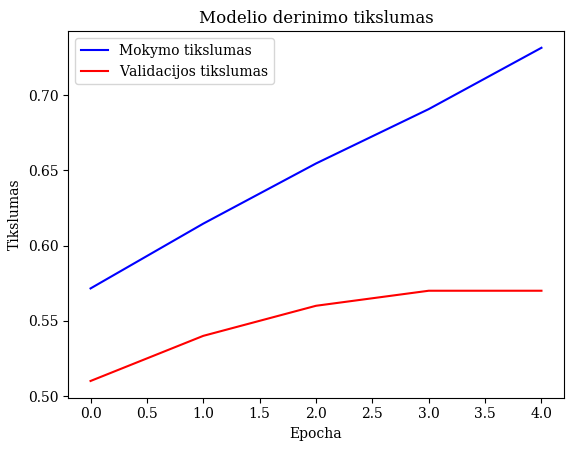
\includegraphics[width=\textwidth]{img/GrapthsNEW/Small/animal/5/Acc_DC_S_5.png}
      \caption{NASNetMobile modelio derinimo tikslumas su gyvūnų rinkiniu ir 5 mokymosi sluoksniais}
    \end{minipage}
    \hspace{2mm}
    \begin{minipage}[b]{0.48\textwidth}
      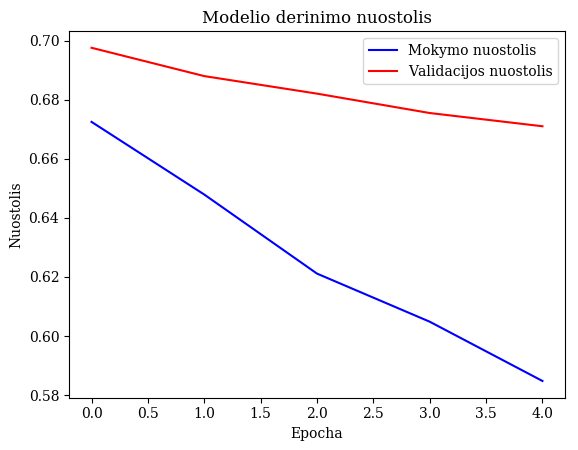
\includegraphics[width=\textwidth]{img/GrapthsNEW/Small/animal/5/Loss_DC_S_5.png}
      \caption{NASNetMobile modelio derinimo nuostolis su gyvūnų rinkiniu ir 5 mokymosi sluoksniais}
    \end{minipage}
\end{figure}

\begin{figure}[!htbp]
    \centering
    \begin{minipage}[b]{0.48\textwidth}
      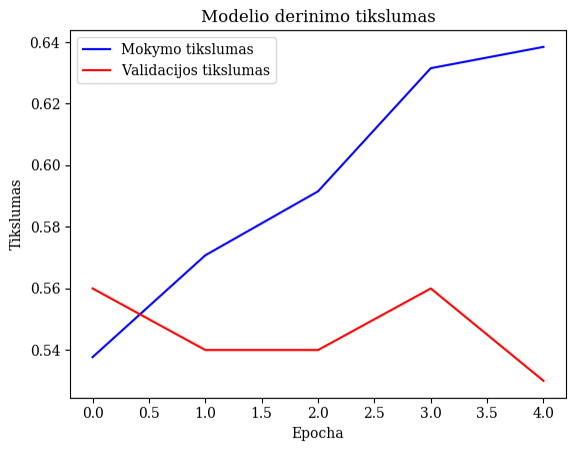
\includegraphics[width=\textwidth]{img/GrapthsNEW/Small/room/5/Acc_R_S_5.png}
      \caption{NASNetMobile modelio derinimo tikslumas su kambarių rinkiniu ir 5 mokymosi sluoksniais}
    \end{minipage}
    \hspace{2mm}
    \begin{minipage}[b]{0.48\textwidth}
      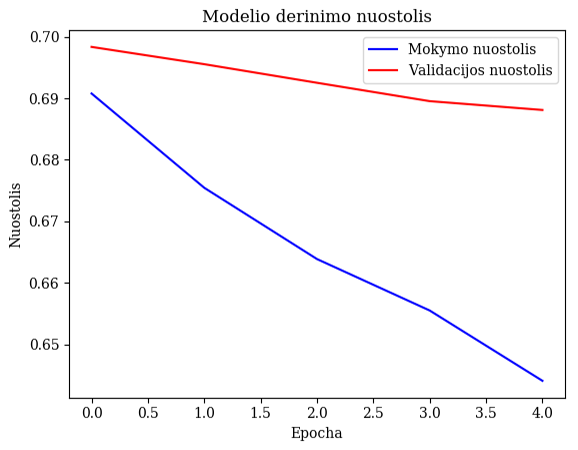
\includegraphics[width=\textwidth]{img/GrapthsNEW/Small/room/5/Loss_R_S_5.png}
      \caption{NASNetMobile modelio derinimo nuostolis su kambarių rinkiniu ir 5 mokymosi sluoksniais}
    \end{minipage}
\end{figure}
% -------------------------------------------------------------------------------------------
% -------------------------------------------------------------------------------------------
\begin{figure}[!htbp]
    \centering
    \begin{minipage}[b]{0.48\textwidth}
      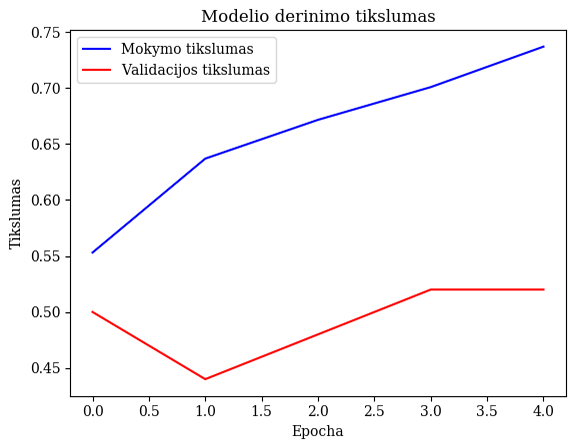
\includegraphics[width=\textwidth]{img/GrapthsNEW/Small/animal/10/Acc_DC_S_10.png}
      \caption{NASNetMobile modelio derinimo tikslumas su gyvūnų rinkiniu ir 10 mokymosi sluoksnių}
    \end{minipage}
    \hspace{2mm}
    \begin{minipage}[b]{0.48\textwidth}
      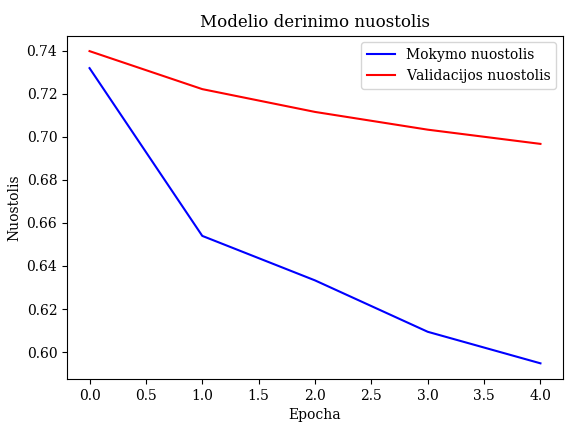
\includegraphics[width=\textwidth]{img/GrapthsNEW/Small/animal/10/Loss_DC_S_10.png}
      \caption{NASNetMobile modelio derinimo nuostolis su gyvūnų rinkiniu ir 10 mokymosi sluoksnių}
    \end{minipage}
\end{figure}

\begin{figure}[!htbp]
    \centering
    \begin{minipage}[b]{0.48\textwidth}
      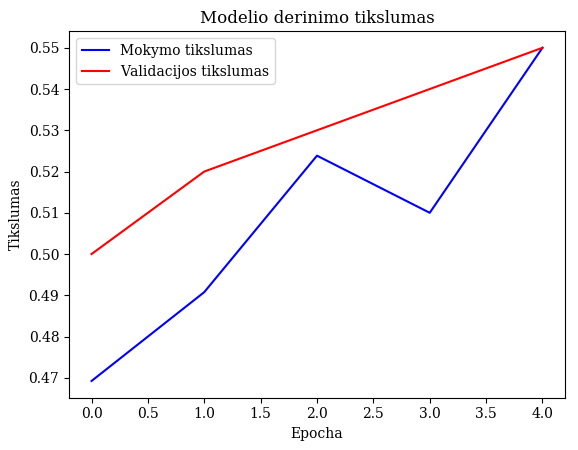
\includegraphics[width=\textwidth]{img/GrapthsNEW/Small/room/10/Acc_R_S_10.png}
      \caption{NASNetMobile modelio derinimo tikslumas su kambarių rinkiniu ir 10 mokymosi sluoksnių}
    \end{minipage}
    \hspace{2mm}
    \begin{minipage}[b]{0.48\textwidth}
      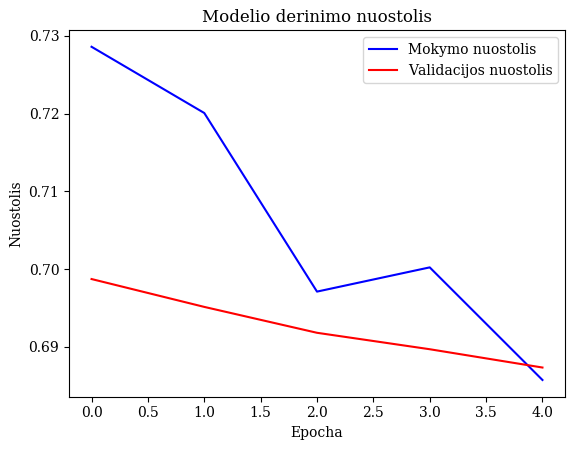
\includegraphics[width=\textwidth]{img/GrapthsNEW/Small/room/10/Loss_R_S_10.png}
      \caption{NASNetMobile modelio derinimo nuostolis su kambarių rinkiniu ir 10 mokymosi sluoksnių}
    \end{minipage}
\end{figure}
% -------------------------------------------------------------------------------------------
% -------------------------------------------------------------------------------------------
\begin{figure}[!htbp]
    \centering
    \begin{minipage}[b]{0.48\textwidth}
      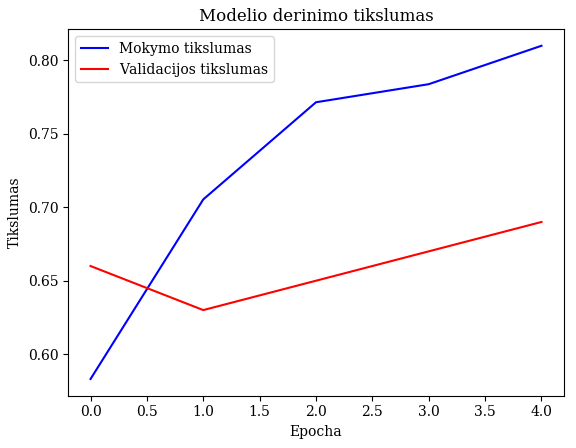
\includegraphics[width=\textwidth]{img/GrapthsNEW/Small/animal/20/Acc_DC_S_20.png}
      \caption{NASNetMobile modelio derinimo tikslumas su gyvūnų rinkiniu ir 20 mokymosi sluoksnių}
    \end{minipage}
    \hspace{2mm}
    \begin{minipage}[b]{0.48\textwidth}
      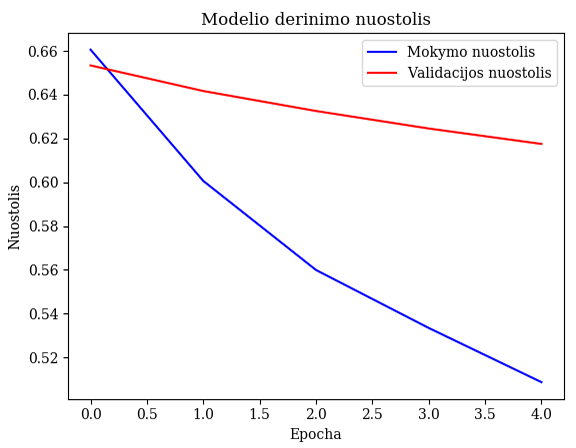
\includegraphics[width=\textwidth]{img/GrapthsNEW/Small/animal/20/Loss_DC_S_20.png}
      \caption{NASNetMobile modelio derinimo nuostolis su gyvūnų rinkiniu ir 20 mokymosi sluoksnių}
    \end{minipage}
\end{figure}

\begin{figure}[!htbp]
    \centering
    \begin{minipage}[b]{0.48\textwidth}
      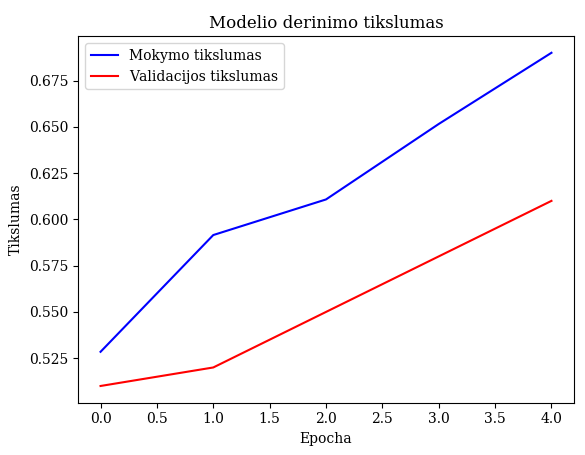
\includegraphics[width=\textwidth]{img/GrapthsNEW/Small/room/20/Acc_R_S_20.png}
      \caption{NASNetMobile modelio derinimo tikslumas su kambarių rinkiniu ir 20 mokymosi sluoksnių}
    \end{minipage}
    \hspace{2mm}
    \begin{minipage}[b]{0.48\textwidth}
      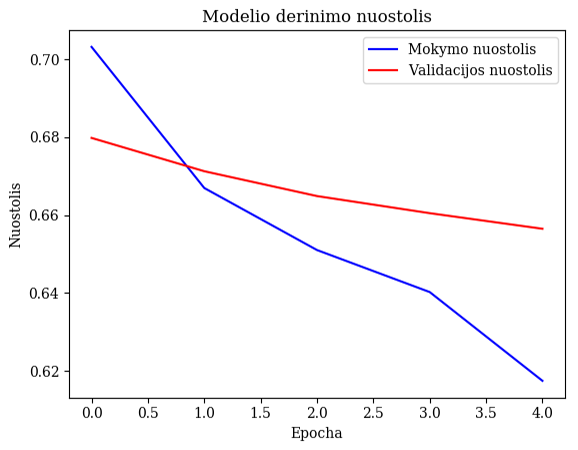
\includegraphics[width=\textwidth]{img/GrapthsNEW/Small/room/20/Loss_R_S_20.png}
      \caption{NASNetMobile modelio derinimo nuostolis su kambarių rinkiniu ir 20 mokymosi sluoksnių}
    \end{minipage}
\end{figure}
% -------------------------------------------------------------------------------------------
% -------------------------------------------------------------------------------------------
% -------------------------------------------------------------------------------------------

\begin{figure}[!htbp]
    \centering
    \begin{minipage}[b]{0.48\textwidth}
      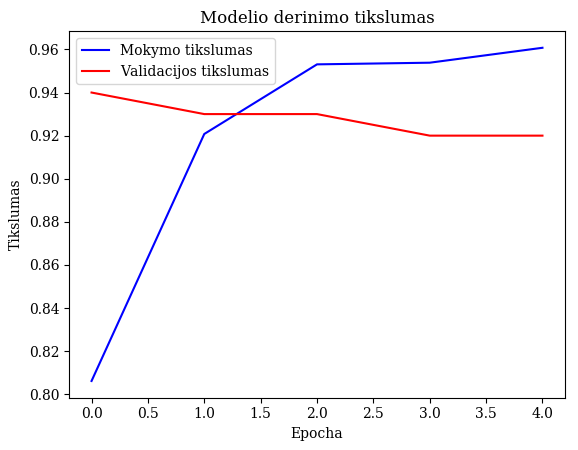
\includegraphics[width=\textwidth]{img/GrapthsNEW/Large/animal/5/Acc_DC_L_5.png}
      \caption{NASNetLarge modelio derinimo tikslumas su gyvūnų rinkiniu ir 5 mokymosi sluoksniais}
    \end{minipage}
    \hspace{2mm}
    \begin{minipage}[b]{0.48\textwidth}
      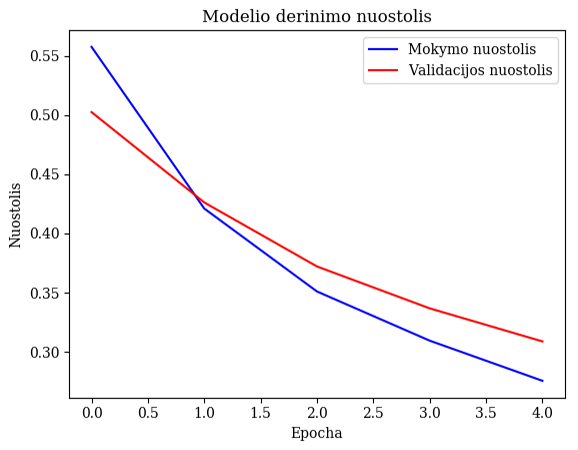
\includegraphics[width=\textwidth]{img/GrapthsNEW/Large/animal/5/Loss_DC_L_5.png}
      \caption{NASNetLarge modelio derinimo nuostolis su gyvūnų rinkiniu ir 5 mokymosi sluoksniais}
    \end{minipage}
\end{figure}

\begin{figure}[!htbp]
    \centering
    \begin{minipage}[b]{0.48\textwidth}
      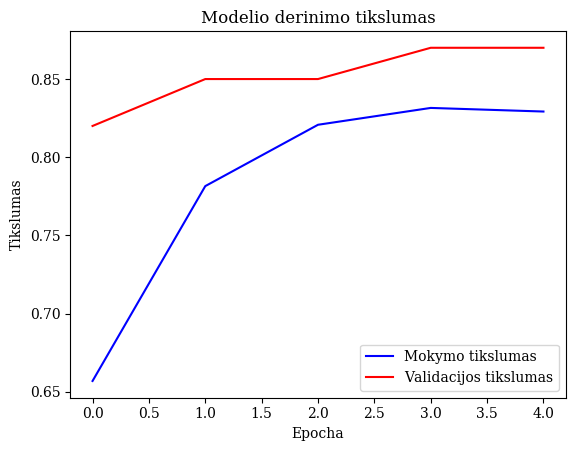
\includegraphics[width=\textwidth]{img/GrapthsNEW/Large/room/5/Acc_R_L_5.png}
      \caption{NASNetLarge modelio derinimo tikslumas su kambarių rinkiniu ir 5 mokymosi sluoksniais}
    \end{minipage}
    \hspace{2mm}
    \begin{minipage}[b]{0.48\textwidth}
      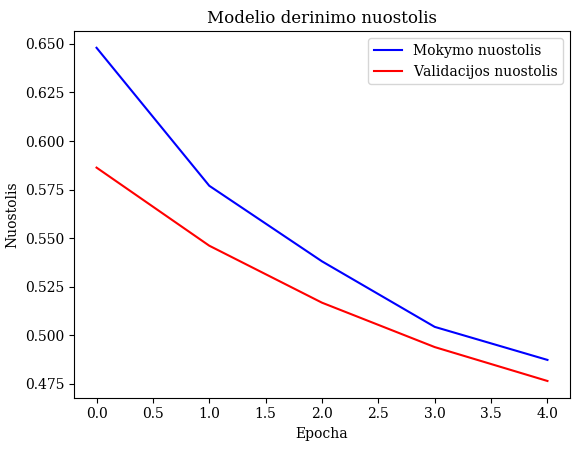
\includegraphics[width=\textwidth]{img/GrapthsNEW/Large/room/5/Loss_R_L_5.png}
      \caption{NASNetLarge modelio derinimo nuostolis su kambarių rinkiniu ir 5 mokymosi sluoksniais}
    \end{minipage}
\end{figure}
% -------------------------------------------------------------------------------------------
% -------------------------------------------------------------------------------------------
\begin{figure}[!htbp]
    \centering
    \begin{minipage}[b]{0.48\textwidth}
      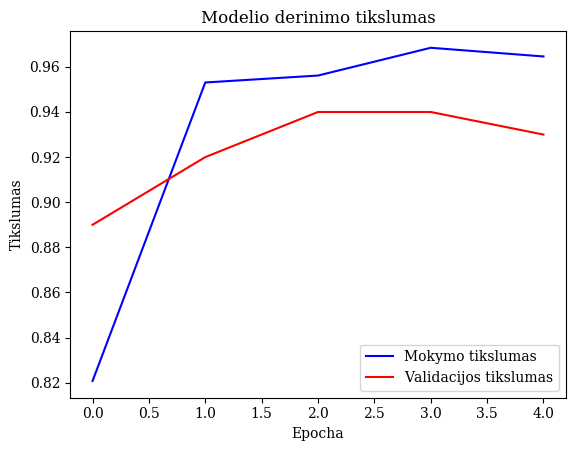
\includegraphics[width=\textwidth]{img/GrapthsNEW/Large/animal/10/Acc_DC_L_10.png}
      \caption{NASNetLarge modelio derinimo tikslumas su gyvūnų rinkiniu ir 10 mokymosi sluoksnių}
    \end{minipage}
    \hspace{2mm}
    \begin{minipage}[b]{0.48\textwidth}
      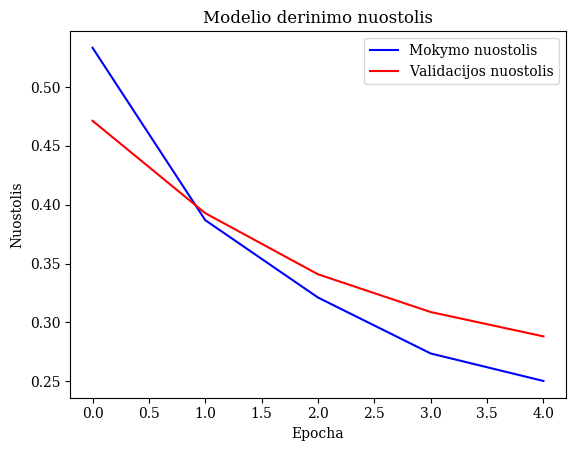
\includegraphics[width=\textwidth]{img/GrapthsNEW/Large/animal/10/Loss_DC_L_10.png}
      \caption{NASNetLarge modelio derinimo nuostolis su gyvūnų rinkiniu ir 10 mokymosi sluoksnių}
    \end{minipage}
\end{figure}

\begin{figure}[!htbp]
    \centering
    \begin{minipage}[b]{0.48\textwidth}
      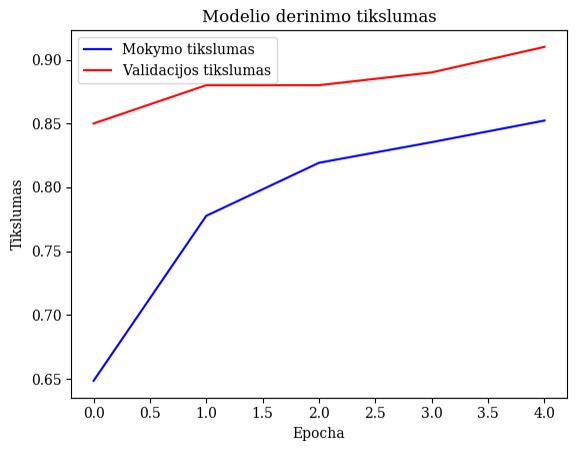
\includegraphics[width=\textwidth]{img/GrapthsNEW/Large/room/10/Acc_R_L_10.png}
      \caption{NASNetLarge modelio derinimo tikslumas su kambarių rinkiniu ir 10 mokymosi sluoksnių}
    \end{minipage}
    \hspace{2mm}
    \begin{minipage}[b]{0.48\textwidth}
      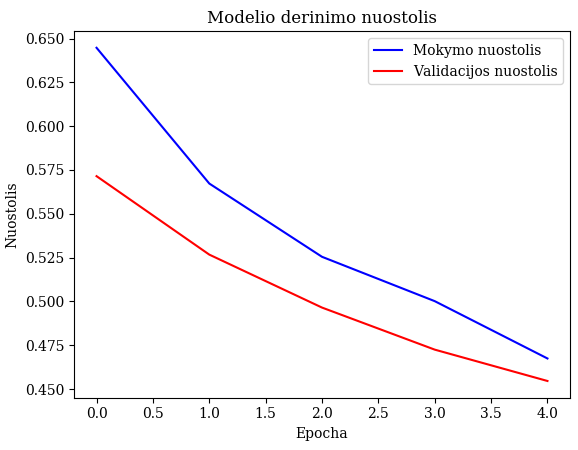
\includegraphics[width=\textwidth]{img/GrapthsNEW/Large/room/10/Loss_R_L_10.png}
      \caption{NASNetLarge modelio derinimo nuostolis su kambarių rinkiniu ir 10 mokymosi sluoksnių}
    \end{minipage}
\end{figure}
% -------------------------------------------------------------------------------------------
% -------------------------------------------------------------------------------------------
\begin{figure}[!htbp]
    \centering
    \begin{minipage}[b]{0.48\textwidth}
      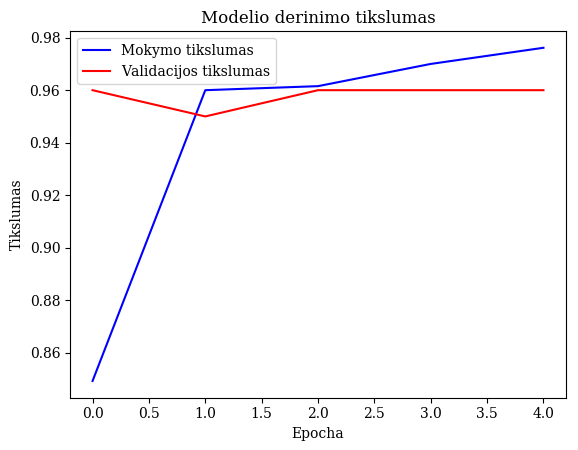
\includegraphics[width=\textwidth]{img/GrapthsNEW/Large/animal/20/Acc_DC_L_20.png}
      \caption{NASNetLarge modelio derinimo tikslumas su gyvūnų rinkiniu ir 20 mokymosi sluoksnių}
    \end{minipage}
    \hspace{2mm}
    \begin{minipage}[b]{0.48\textwidth}
      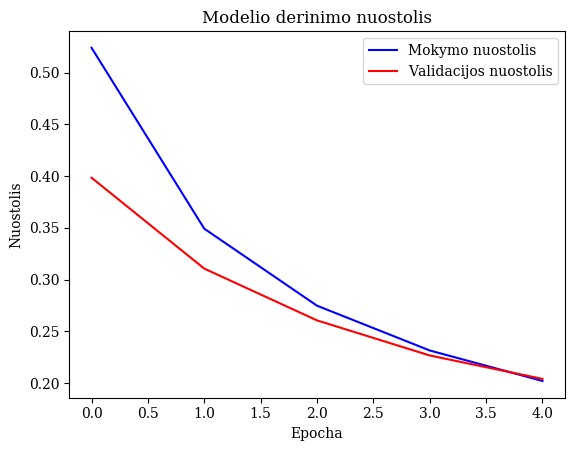
\includegraphics[width=\textwidth]{img/GrapthsNEW/Large/animal/20/Loss_DC_L_20.png}
      \caption{NASNetLarge modelio derinimo nuostolis su gyvūnų rinkiniu ir 20 mokymosi sluoksnių}
    \end{minipage}
\end{figure}

\begin{figure}[H]
    \centering
    \begin{minipage}[b]{0.48\textwidth}
      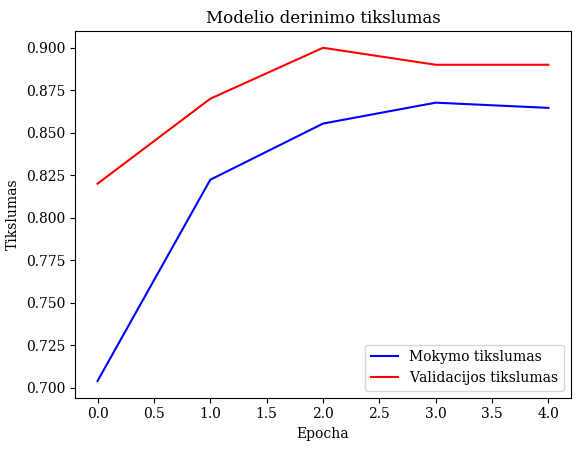
\includegraphics[width=\textwidth]{img/GrapthsNEW/Large/room/20/Acc_R_L_20.png}
      \caption{NASNetLarge modelio derinimo tikslumas su kambarių rinkiniu ir 20 mokymosi sluoksnių}
    \end{minipage}
    \hspace{2mm}
    \begin{minipage}[b]{0.48\textwidth}
      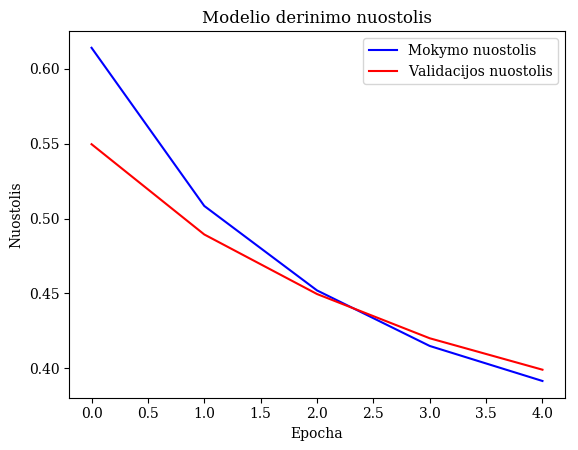
\includegraphics[width=\textwidth]{img/GrapthsNEW/Large/room/20/Loss_R_L_20.png}
      \caption{NASNetLarge modelio derinimo nuostolis su kambarių rinkiniu ir 20 mokymosi sluoksnių}
    \end{minipage}
\end{figure}
\end{document}
